%==============================================================================00
% Options for packages loaded elsewhere
\PassOptionsToPackage{unicode}{hyperref}
\PassOptionsToPackage{hyphens}{url}
%==============================================================================01
\documentclass[11pt, oneside, openany]{scrbook}
\setkomafont{disposition}{\bfseries}
\usepackage{mathptmx}
\usepackage{lipsum}
%==============================================================================03
% Make chapter pages have numbering at top right
\usepackage{fancyhdr}
\pagestyle{fancy}
\lhead{}
\chead{}
\rhead{\thepage}
\lfoot{}
\cfoot{}
\rfoot{}
\renewcommand{\headrulewidth}{0pt}
\makeatletter
\renewcommand\chapter{\if@openright\cleardoublepage\else\clearpage\fi
                    \thispagestyle{fancy}%
                    \global\@topnum\z@
                    \@afterindentfalse
                    \secdef\@chapter\@schapter}
\makeatother
%==============================================================================03
\usepackage{lmodern}
\usepackage{setspace}
%==============================================================================04
\usepackage{amssymb,amsmath}
%==============================================================================05
\usepackage{ifxetex,ifluatex}
\ifnum 0\ifxetex 1\fi\ifluatex 1\fi=0 % if pdftex
  \usepackage[T1]{fontenc}
  \usepackage[utf8]{inputenc}
  \usepackage{textcomp} % provide euro and other symbols
\else % if luatex or xetex
  \usepackage{unicode-math}
  \defaultfontfeatures{Scale=MatchLowercase}
  \defaultfontfeatures[\rmfamily]{Ligatures=TeX,Scale=1}
\fi
%==============================================================================06
% Use upquote if available, for straight quotes in verbatim environments
\IfFileExists{upquote.sty}{\usepackage{upquote}}{}
\IfFileExists{microtype.sty}{% use microtype if available
  \usepackage[]{microtype}
  \UseMicrotypeSet[protrusion]{basicmath} % disable protrusion for tt fonts
}{}
\makeatletter
\@ifundefined{KOMAClassName}{% if non-KOMA class
  \IfFileExists{parskip.sty}{%
    \usepackage{parskip}
  }{% else
    \setlength{\parindent}{0pt}
    \setlength{\parskip}{6pt plus 2pt minus 1pt}}
}{% if KOMA class
  \KOMAoptions{parskip=half}}
\makeatother
%==============================================================================07
\usepackage[table]{xcolor}
%==============================================================================08
\IfFileExists{xurl.sty}{\usepackage{xurl}}{} % add URL line breaks if available
\IfFileExists{bookmark.sty}{\usepackage{bookmark}}{\usepackage{hyperref}}
\hypersetup{
  pdftitle={Application of a Principaled Bayesian Workflow to Multilevel Modeling},
  pdfauthor={Alexander D. Knudson},
  hidelinks,
  pdfcreator={LaTeX via pandoc}}
\urlstyle{same} % disable monospaced font for URLs
%==============================================================================09
\usepackage[top=1in, left=1.5in, bottom=1.25in, right=1.5in]{geometry}
%==============================================================================10
\usepackage{color}
\usepackage{fancyvrb}
\newcommand{\VerbBar}{|}
\newcommand{\VERB}{\Verb[commandchars=\\\{\}]}
\DefineVerbatimEnvironment{Highlighting}{Verbatim}{commandchars=\\\{\}}
% Add ',fontsize=\small' for more characters per line
\usepackage{framed}
\definecolor{shadecolor}{RGB}{248,248,248}
\newenvironment{Shaded}{\begin{snugshade}}{\end{snugshade}}
\newcommand{\AlertTok}[1]{\textcolor[rgb]{0.94,0.16,0.16}{#1}}
\newcommand{\AnnotationTok}[1]{\textcolor[rgb]{0.56,0.35,0.01}{\textbf{\textit{#1}}}}
\newcommand{\AttributeTok}[1]{\textcolor[rgb]{0.77,0.63,0.00}{#1}}
\newcommand{\BaseNTok}[1]{\textcolor[rgb]{0.00,0.00,0.81}{#1}}
\newcommand{\BuiltInTok}[1]{#1}
\newcommand{\CharTok}[1]{\textcolor[rgb]{0.31,0.60,0.02}{#1}}
\newcommand{\CommentTok}[1]{\textcolor[rgb]{0.56,0.35,0.01}{\textit{#1}}}
\newcommand{\CommentVarTok}[1]{\textcolor[rgb]{0.56,0.35,0.01}{\textbf{\textit{#1}}}}
\newcommand{\ConstantTok}[1]{\textcolor[rgb]{0.00,0.00,0.00}{#1}}
\newcommand{\ControlFlowTok}[1]{\textcolor[rgb]{0.13,0.29,0.53}{\textbf{#1}}}
\newcommand{\DataTypeTok}[1]{\textcolor[rgb]{0.13,0.29,0.53}{#1}}
\newcommand{\DecValTok}[1]{\textcolor[rgb]{0.00,0.00,0.81}{#1}}
\newcommand{\DocumentationTok}[1]{\textcolor[rgb]{0.56,0.35,0.01}{\textbf{\textit{#1}}}}
\newcommand{\ErrorTok}[1]{\textcolor[rgb]{0.64,0.00,0.00}{\textbf{#1}}}
\newcommand{\ExtensionTok}[1]{#1}
\newcommand{\FloatTok}[1]{\textcolor[rgb]{0.00,0.00,0.81}{#1}}
\newcommand{\FunctionTok}[1]{\textcolor[rgb]{0.00,0.00,0.00}{#1}}
\newcommand{\ImportTok}[1]{#1}
\newcommand{\InformationTok}[1]{\textcolor[rgb]{0.56,0.35,0.01}{\textbf{\textit{#1}}}}
\newcommand{\KeywordTok}[1]{\textcolor[rgb]{0.13,0.29,0.53}{\textbf{#1}}}
\newcommand{\NormalTok}[1]{#1}
\newcommand{\OperatorTok}[1]{\textcolor[rgb]{0.81,0.36,0.00}{\textbf{#1}}}
\newcommand{\OtherTok}[1]{\textcolor[rgb]{0.56,0.35,0.01}{#1}}
\newcommand{\PreprocessorTok}[1]{\textcolor[rgb]{0.56,0.35,0.01}{\textit{#1}}}
\newcommand{\RegionMarkerTok}[1]{#1}
\newcommand{\SpecialCharTok}[1]{\textcolor[rgb]{0.00,0.00,0.00}{#1}}
\newcommand{\SpecialStringTok}[1]{\textcolor[rgb]{0.31,0.60,0.02}{#1}}
\newcommand{\StringTok}[1]{\textcolor[rgb]{0.31,0.60,0.02}{#1}}
\newcommand{\VariableTok}[1]{\textcolor[rgb]{0.00,0.00,0.00}{#1}}
\newcommand{\VerbatimStringTok}[1]{\textcolor[rgb]{0.31,0.60,0.02}{#1}}
\newcommand{\WarningTok}[1]{\textcolor[rgb]{0.56,0.35,0.01}{\textbf{\textit{#1}}}}
%==============================================================================11
\usepackage{longtable,booktabs}
\usepackage{multirow}
% Correct order of tables after \paragraph or \subparagraph
\usepackage{etoolbox}
\makeatletter
\patchcmd\longtable{\par}{\if@noskipsec\mbox{}\fi\par}{}{}
\makeatother
% Allow footnotes in longtable head/foot
\IfFileExists{footnotehyper.sty}{\usepackage{footnotehyper}}{\usepackage{footnote}}
\makesavenoteenv{longtable}
%==============================================================================12
\usepackage{graphicx}
\makeatletter
\def\maxwidth{\ifdim\Gin@nat@width>\linewidth\linewidth\else\Gin@nat@width\fi}
\def\maxheight{\ifdim\Gin@nat@height>\textheight\textheight\else\Gin@nat@height\fi}
\makeatother
% Scale images if necessary, so that they will not overflow the page
% margins by default, and it is still possible to overwrite the defaults
% using explicit options in \includegraphics[width, height, ...]{}
\setkeys{Gin}{width=\maxwidth,height=\maxheight,keepaspectratio}
% Set default figure placement to htbp
\makeatletter
\def\fps@figure{htbp}
\makeatother
%==============================================================================13
%==============================================================================14
%==============================================================================15
\setlength{\emergencystretch}{3em} % prevent overfull lines
\providecommand{\tightlist}{%
  \setlength{\itemsep}{0pt}\setlength{\parskip}{0pt}}
%==============================================================================16
\setcounter{secnumdepth}{5}
%==============================================================================17
%==============================================================================18
% Place here anything extra that you would like in the preamble
%==============================================================================19
\ifluatex
  \usepackage{selnolig}  % disable illegal ligatures
\fi
%==============================================================================20
\usepackage[]{natbib}
\bibliographystyle{apalike}
%==============================================================================21
\frontmatter

\begin{document}

\begin{titlepage}
\begin{center}
\vspace*{1in}
University of Nevada, Reno

\vspace{1.5in}
\textbf{Application of a Principaled Bayesian Workflow to Multilevel Modeling}

\vspace{1in}
A thesis submitted in partial fulfillment of the \\
requirements for the degree of Master of Science in \\
Statistics and Data Science

\vspace{1in}
by

\vspace{1em}
Alexander D. Knudson

\vspace{2em}
A.G. Schissler

\vspace{3em}
December, 2020

\end{center}
\end{titlepage}
%==============================================================================22
% Begin Copyright --------------------- (optional)
\thispagestyle{empty}
\begin{center}
\vspace*{\fill}
Copyright by Albert Einstein 1944 \\
All Rights Reserved
\vspace*{\fill}
\end{center}
%------------------------ End Copyright


% Begin Committee Approval Page -------
\newpage
\thispagestyle{empty}
\begin{center}


\includegraphics[width=0.75in, height=0.75in]{./figures/unr_logos/University Logo RGB_block_n_blue}

THE GRADUATE SCHOOL

\vspace{1em}
We recommend that the thesis \\
prepared under our supervision by\\

\vspace{1em}
\textbf{Alexander Knudson}

\vspace{1em}
entitled

\textbf{THESIS TITLE}

\vspace{2em}
be accepted in partial fullfilment of the \\
requirements for the degree of

\vspace{1em}
\textbf{Master of Science}

\vspace{1em}
Dr. A.G. Schissler \\
\textit{Advisor}

\vspace{1em}
Dr. Colin Grudzien\\
\textit{Committee Member}

\vspace{1em}
Dr. Fang Jiang \\
\textit{Graduate School Representative}

\vspace{1em}
David W. Zeh, Ph.D., Dean \\
\textit{Graduate School}

\vspace{1em}
August, 2020
\end{center}
%---------- End Committee Approval Page


% Begin ---------------
\newpage
\setcounter{page}{1} % Begin lower case Roman numerals
\section*{Abstract}
\lipsum[1]
%------------------ End


% Begin ---------------
\newpage
\section*{Dedication (optional)}
\lipsum[2-3]
%------------------ End


% Begin ---------------
\newpage
\section*{Acknowledgments (optional)}
\lipsum[4]
%------------------ End

% Begin ---------------
\setcounter{tocdepth}{1}
\tableofcontents

\listoftables

\listoffigures
%------------------ End
%==============================================================================23
\setstretch{2.0}
%==============================================================================24
\mainmatter
%==============================================================================25
\hypertarget{intro}{%
\chapter{Introduction}\label{intro}}

With the advances in computational power and high-level programming languages like Python, R, and Julia, statistical methods have evolved to be more flexible and expressive. No longer must we be subjugated by p-values and step-wise regression techniques. Gone are the days of using clever modeling techniques to tame misbehaved data. Now is the time for principled and informed decisions to create bespoke models and domain-motivated analyses. We have the shoulders of giants to stand upon and look out at the vast sea of data science.

I want to talk about how the advances in computational power have lead to a sort of mini revolution - resurrection - in statistics where Bayesian modeling has gained an incredible following thanks to projects like Stan. The steady adoption of computer aided statistical workflows also brings the need for multidisciplinary techniques from numerical analysis, probability theory, statistics, computer science, visualizations, and more. And with the age of computers, there is a strong push towards reproducibility. Concepts of modular design, workflows, project history and versioning, virtual environments, and human readable code all contribute to reproducible analyses. And somehow I also want to tie in how data is immutable - raw data should (must) be treated as a constant and unchangeable entity, and merely touching it will cause data mitosis.

I will now segue into introducing the intent of this paper. I believe that utilizing the computational ability of modern computers helps strengthen the validity of an analysis. This is achieved by using powerful but expressive tools like Stan to write models that visually match written mathematical models. Classical statistical tools, while fast, require clever mathematics to perform certain routines such as fitting mixed effects models or the interpretation of cryptic p-values to determine if a model is ``good''. Instead I believe we should be moving towards probabilistic programming languages like Stan to carry out Statistical analyses.

This paper is motivated by an experiment in psychometrics (\protect\hyperlink{motivating-data}{chapter 2}), and by highlighting a principled workflow I seek to convince the reader that Bayesian multilevel modeling should be the default tool for modeling psychometric experiments. In the next section of this introduction, I will list classical tools for statistical modeling {[}of psychometric experiments{]} and touch on the limitations of such tools. Following that section, I will introduce the methods I use for building a model that deviate from classical methods.

\hypertarget{ch010-classical-methods}{%
\section{Everything can be Blamed on Fisher}\label{ch010-classical-methods}}

\emph{\ldots{} or Pearson, or Gauss, or \ldots{}}

When I hear the term ``regression'', I instantly think about maximum likelihood estimation (MLE) of parameters. And why not? There is an endless wealth of literature on the subject of linear regression and MLE \citep{johnson2002applied, larsen2005introduction, sheather2009modern, navidi2015statistics}. Most introductory courses on statistics and regression center around classical techniques such as MLE, hypothesis testing, and residual analysis. For the common student, learning statistical modeling in classical way can feel sterilized and mechanic. Check that the data are normal. Check that the coefficients are significantly different from zero. Check that the residuals are normal. Etc. I'm not trying to say that these methods are not important or that they are deeply flawed - it would be bad for modern society if we were just now finding out that the models are wrong. Instead, I am arguing that because they are so common and easy to apply that they are used without much extra thought.

Take variable selection as an example. In a data set where there are a dozen predictors, how does one go about selecting which parameters produce the best model? Without thought, one may reach for a step-wise selection algorithm, and confidently conclude that variables \(x\), \(y\), and \(z\) are \emph{significant} because the p-values say so. This method does fall apart quickly because as the number of parameters grow, so too does the number of steps needed to find the best subset of variables\footnote{The number of subsets grows exponentially with the number of parameters. Forward and backward selection steps grows quadratically.}, and there is no guarantee that the algorithm actually selects the best\footnote{I'm being intentionally vague about what I mean by ``best'' because what is best is determined by the application} subset. But even if the best subset of variables is found, one still needs to consider if the variables have a practical effect or if the model omitted an important variable of interest.

Sure, the type of analysis is important to the techniques used. Variable selection through step-wise algorithms or penalized maximum likelihood estimation \citep{hoerl1970ridge, tibshirani1996regression} may be appropriate in an exploratory data analysis, but improper for causal inference and other scientifically motivated experiments.

Which brings me to talk next about p-values, confidence intervals, and hypothesis testing. The concept of basing scientific results on the falsifiability \citep{popper1959logic} or refutability of a claim is a strong foundation for the scientific method, and is arguably much better than the previous grounds of verifiability -- just because something has been true for a very long time, doesn't mean it will always be true in the future. But hypothesis testing comes with its own set of problems. Null hypothesis testing for point estimates usually depends on calculating a confidence interval and seeing if the interval contains the point of interest. This can be misleading, as there is more than one confidence interval that can be calculated. For Gaussian distributions, the mean equals the median equals the mode, so a 95\% confidence interval is evenly distributed around the central measures. Some distributions are skewed, so an equal tail area confidence interval might not necessarily include the most likely value. Take for example the exponential distribution

\[
X \sim \mathrm{exponential} (\lambda)
\]

An equal tail area 95\% confidence interval would be \(\left(-\ln(0.975)/\lambda, -\ln(0.025)/\lambda\right)\) which would not even contain the most likely value of zero. Should the highest density interval be used? Should skewness be reported with p-values and confidence intervals? Furthermore, confidence intervals are conditional on the model chosen, and that introduces other problems. \citet{mcelreath2020statistical} discusses a well-known issue in population biology about comparing a neutral model of the distribution of allele frequencies to a selective model. In short, the two differing hypotheses may suggest different process models which in turn lead to statistical models - some of which are shared by both hypotheses. Rejecting the statistical model doesn't rule out either of the hypotheses.

Should we scrap these principles and tools all together? Absolutely not. Most of these wrinkled problems (and others) have been talked about and ironed out through careful discussion and clever techniques, but the damage is done, and hypothesis testing and p-values are widely misunderstood and misused. The problem is that these techniques rest on having a strong foundation of statistical knowledge, both to produce and to properly understand. This requirement is stifling. Communicating statistical results is just as important as producing them, and with modern tools and a vast selection of expressive languages we can analyze data in a more intuitive and natural framework.

\hypertarget{ch010-new-methods}{%
\section{Proposal of New Methods}\label{ch010-new-methods}}

In my biased opinion, the Bayesian framework for modeling is a much more natural way to conduct scientific research where some kind of data analysis is involved. Now of course, I can't claim as such without some compelling argument or examples. I have already targeted some weak points of classical statistics, and throughout \protect\hyperlink{workflow}{Chapter 3} I will highlight specific examples of where classical techniques are typically applied, and how they may fall short compared to my proposal methods.

What I am proposing is a fully Bayesian workflow to build and analyze a statistical model. In this Bayesian workflow (which shall hence be referred to simply as ``workflow'') I will highlight a set of principles that utilize domain expertise, and focus around building a multilevel model. My goal is to show that the combination of these two concepts yields better prediction results and greater inferential power. And in lieu of p-values and hypothesis testing, I let predictive inference narrate the statistical results and strength of association within the model.

\hypertarget{ch010-organization}{%
\section{Organization}\label{ch010-organization}}

I have organized this thesis as follows. In \protect\hyperlink{motivating-data}{Chapter 2} I introduce the data set that drives the narrative and that motivates the adoption of Bayesian multilevel modeling. In \protect\hyperlink{workflow}{Chapter 3} I describe and work through a principled Bayesian workflow for multilevel modeling. \protect\hyperlink{model-checking}{Chapter 4} goes into more depth on checking the model goodness of fit and model diagnostics in a Bayesian setting. In \protect\hyperlink{predictive-inference}{Chapter 5} I demonstrate how to use the Bayesian model from the principled workflow for predictive inference, and use posterior predictive distributions to plot and compare models. Chapters \protect\hyperlink{}{5} and \protect\hyperlink{}{6} go over the quantitative results and discuss the qualitative choices in the workflow. Then I conclude this paper in \protect\hyperlink{conclusion}{Chapter 7}.

\hypertarget{motivating-data}{%
\chapter{What is a Model without Data}\label{motivating-data}}

\emph{What is data without a model}

It was Charles Darwin who in his book \emph{On the Origin of Species} developed the idea that living organisms adapt in order to better survive in their environment. Sir Francis Galton, inspired by Darwin's ideas, became interested in the differences in human beings and in how to measure those differences. Though the dark side of statistics and hubris lead Galton to become a pioneer of eugenics, his works on studying and measuring human differences lead to the creation of psychometrics -- the science of measuring mental faculties. Around the same time that he was developing his theories, Johann Friedrich Herbart was also interested in studying consciousness through the scientific method, and is responsible for creating mathematical models of the mind.

E.H. Weber built upon Herbart's work, and sought out to prove the idea of a \emph{psychological threshold}. A psychological threshold is a minimum stimulus intensity necessary to activate a sensory system -- a \emph{liminal} stimulus. He paved the way for experimental psychology and is the namesake of \emph{Weber's Law} -- the change in a stimulus that will be just noticeable is a constant ratio of the original stimulus \citep{britannica2014editors}.

\[
\frac{\Delta I}{I} = k
\]

To put this law into practice, consider holding a 1 kg weight (\(I = 1\)), and further suppose that we can \emph{just} detect the difference between a 1 kg weight and a 1.2 kg weight (\(\Delta I = 0.2\)). Then the constant just noticeable ratio is

\[
k = \frac{0.2}{1} = 0.2
\]

So now if we pick up a 10 kg weight, we should be able to determine how much more mass is required to just detect a difference:

\[
\frac{\Delta I}{10} = 0.2 \Rightarrow \Delta I = 2
\]

The difference between a 10 kg and a 12 kg weight should be just barely perceptible. Notice that the difference in the first set of weights is 0.2 and in the second set it is 2. Our perception of the difference in stimulus intensities is not absolute, but relative. G.T. Fechner devised the law (Weber-Fechner Law) that the strength of a sensation grows as the logarithm of the stimulus intensity.

\[S = K \ln I\]

An example to this law is to consider two light sources, one that is 100 lumens (\(S_1 = K \ln 100\)) and another that is 200 lumens (\(S_2 = K \ln 200\)). The intensity of the second light is not perceived as twice as bright, but only about 1.15 times as bright according to the Weber-Fechner law.

\[\theta = S_2 / S_1 \approx 1.15\]

Notice that the value \(K\) cancels out when calculating the relative intensity, but knowing \(K\) can lead to important psychological insights; insights about differences between persons or groups of people! What biological and contextual factors affect how people perceive different stimuli? How do we measure their perception in a meaningful way? As one might expect, we can collect data from psychometric experiments, fit a model to the data from a family of functions called \emph{psychometric functions}, and inspect key operating characteristics of those functions.

\hypertarget{psycho-experiments}{%
\section{Psychometric Experiments}\label{psycho-experiments}}

Psychometric experiments are devised in a way to examine psychophysical processes, or the response between the world around us and our inward perceptions. A \textbf{psychometric function} relates an observer's performance to an independent variable, usually some physical quantity of a stimulus in a psychophysical task \citep{wichmann2001a}. Psychometric functions were studied as early as the late 1800's, and Edwin Boring published a chart of the psychometric function in The American Journal of Psychology in 1917 \citep{boring1917chart}.

\begin{figure}

{\centering 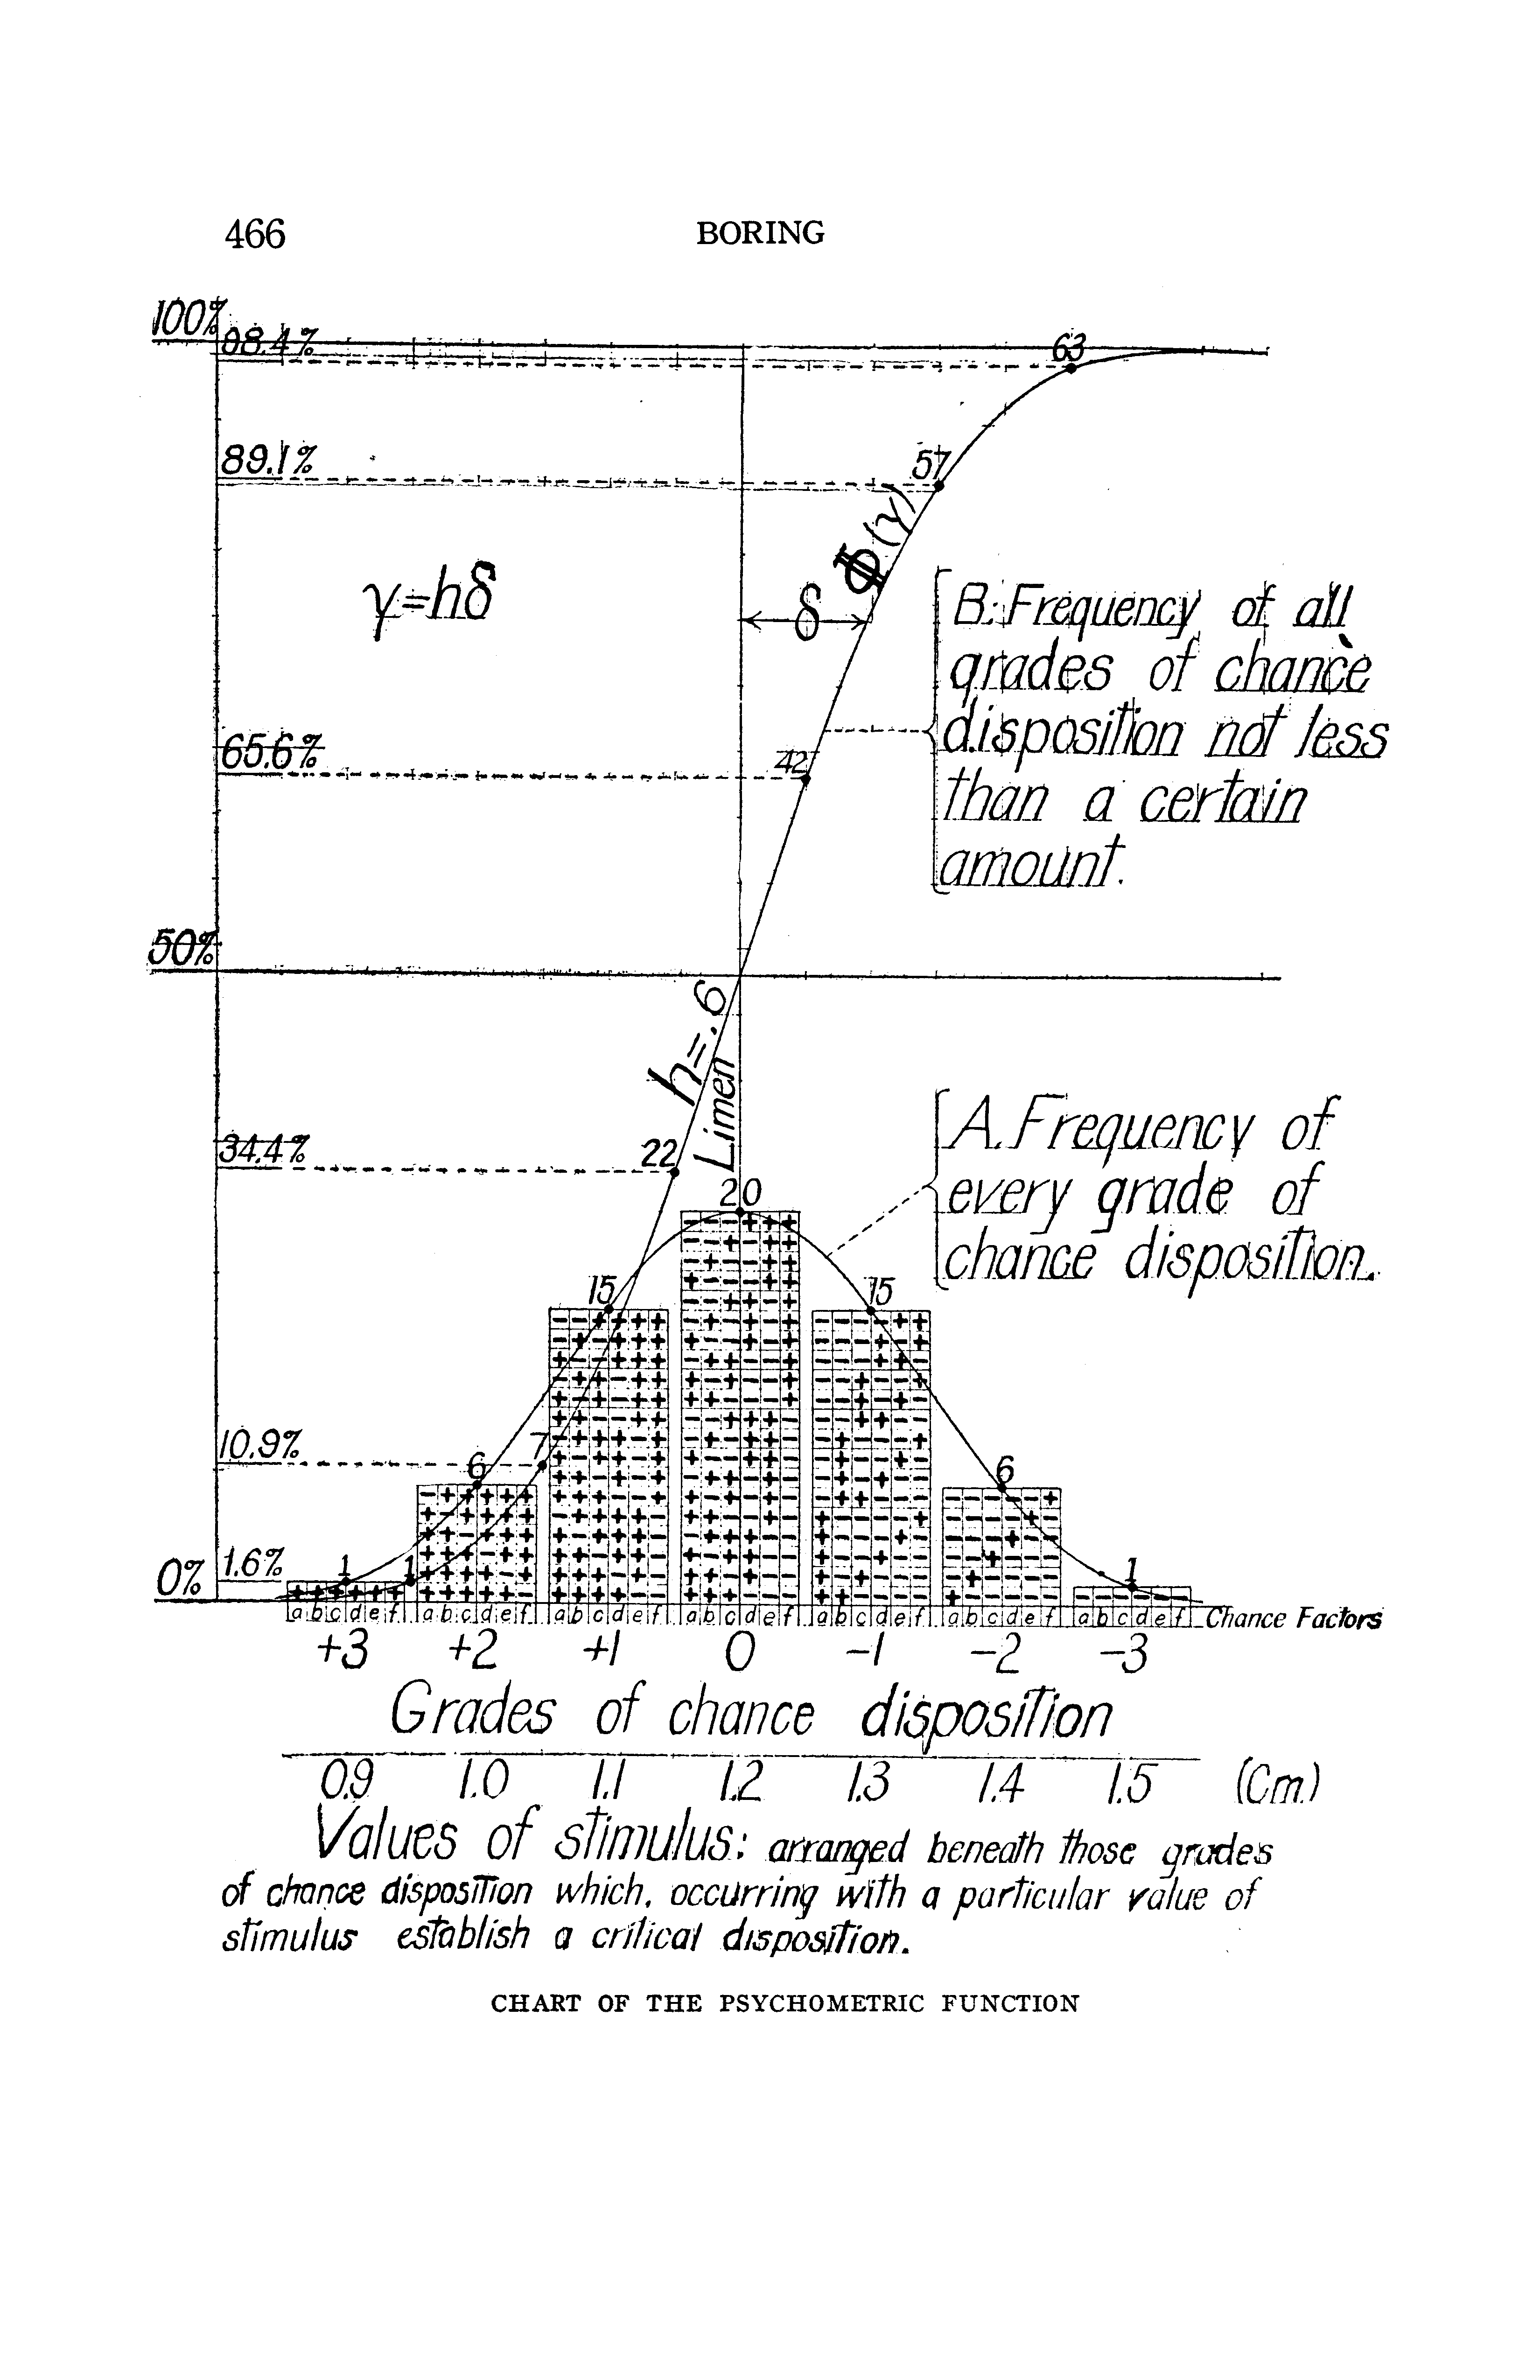
\includegraphics[width=0.7\linewidth]{figures/chart_of_pf} 

}

\caption{A chart of the psychometric function. The experiment in this paper places two points on a subject's skin separated by some distance, and has them answer their impression of whether there is one point or two, recorded as either 'two points' or 'not two points'. As the separation of aesthesiometer points increases, so too does the subject's confidence in their perception of 'two-ness'. So at what separation is the impression of two points liminal?}\label{fig:ch020-chart-of-pf}
\end{figure}

Figure \ref{fig:ch020-chart-of-pf} displays the key aspects of the psychometric function. The most crucial part is the sigmoid function, the S-like non-decreasing curve which in this case is represented by the Normal CDF, \(\Phi(\gamma)\). The horizontal axis represents the stimulus stimulus intensity, the separation of two points in centimeters. The vertical axis represents the probability that a subject has the impression of two points. With only experimental data, the response proportion becomes an approximation for the probability.

This leads me to talk about the type of psychometric experiment that this paper deals with called a \emph{temporal order judgment} (TOJ) experiment. The concept is that if there are two distinct stimuli occurring nearly simultaneously then our brains will bind them into a single percept (perceive them as happening simultaneously). Compensation for small temporal differences is beneficial for coherent multisensory experiences, particularly in visual-speech synthesis as it is necessary to maintain an accurate representation of the sources of multisensory events. The temporal asynchrony between stimuli is called the \emph{stimulus onset asynchrony} (SOA), and the range of SOAs for which sensory signals are integrated into a global percept is called the \emph{temporal binding window}. When the SOA grows too large then the brain segregates the two signals and the temporal order can be determined.

Our experiences in life as we age shape the mechanisms of processing multisensory signals, and some multisensory signals are integrated much more readily than others. Perceptual synchrony has been previously studied through the \emph{point of subjective simultaneity} (PSS) -- the temporal delay between two signals at which an observer is unsure about their temporal order \citep{stone2001now}. The temporal binding window is the time span over which sensory signals arising from different modalities appear integrated into a global percept. A deficit in temporal sensitivity may lead to a widening of the temporal binding window and reduce the ability to segregate unrelated sensory signals. In temporal order judgment tasks, the ability to discriminate the timing of multiple sensory signals is referred to as temporal sensitivity, and is studied through the measurement of the \emph{just noticeable difference} (JND) -- the smallest lapse in time so that a temporal order can just be determined. Figure \ref{fig:ch020-plot-ref-pf} highlights the features through which we study psychometric functions. The PSS is defined as the point where an observer can do no better at determining temporal order than random guessing (i.e.~the response probability is 50\%). The JND is defined as the extra temporal delay between stimuli so that the temporal order is just able to be determined. Historically this has been defined as the difference between the 84\% level\footnote{One standard deviation away from the mean in a Gaussian distribution.} and the PSS, though the upper level often depends on domain expertise.

\begin{figure}

{\centering 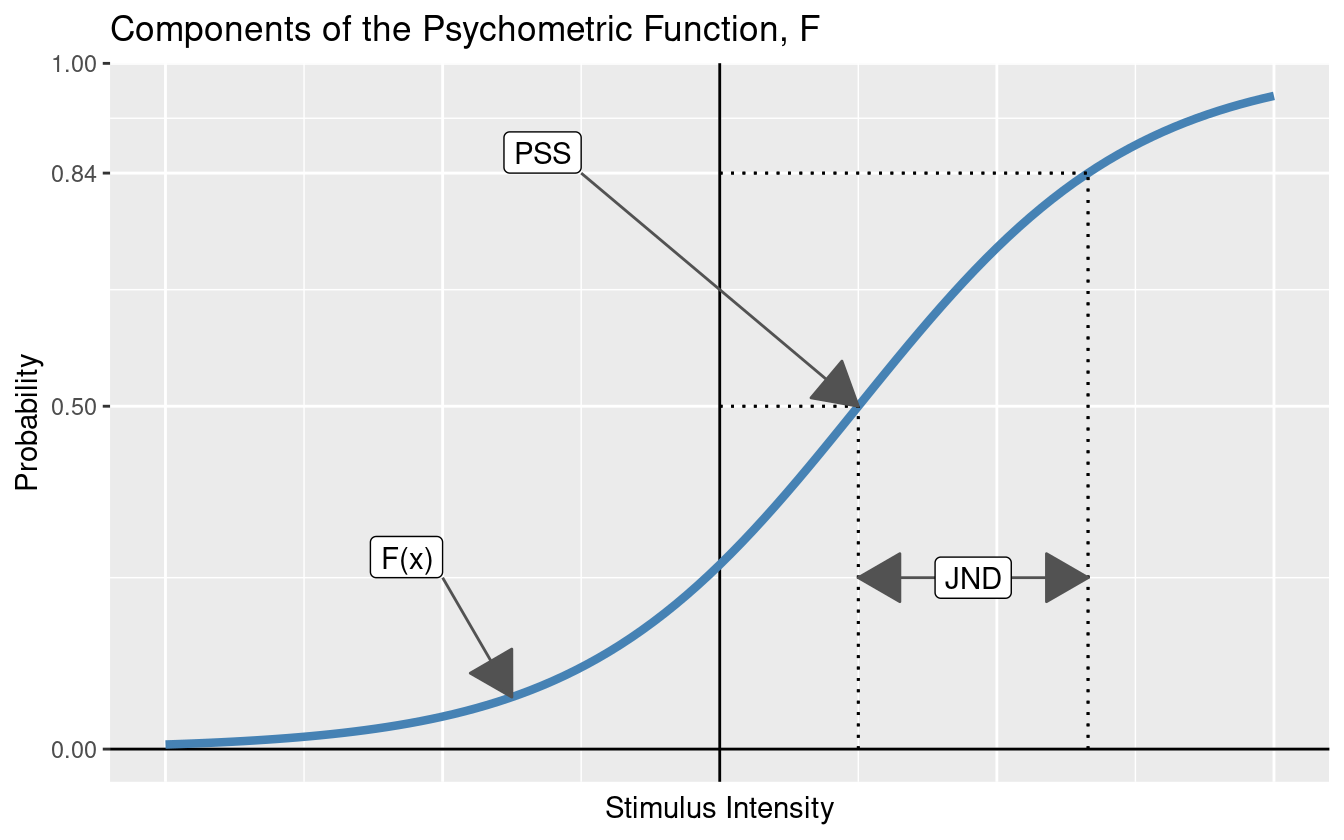
\includegraphics[width=0.7\linewidth]{020-psychometrics_files/figure-latex/ch020-plot-ref-pf-1} 

}

\caption{The PSS is defined as the point where an observer can do no better at determining temporal order than random guessing. The just noticeable difference is defined as the extra temporal delay between stimuli so that the temporal order is just able to be determined. Historically this has been defined as the difference between the 0.84 level and the PSS, though the upper level depends on domain expertise.}\label{fig:ch020-plot-ref-pf}
\end{figure}

Perceptual synchrony and temporal sensitivity can be modified through a baseline understanding. In order to perceive physical events as simultaneous, our brains must adjust for differences in temporal delays of transmission of both psychical signals and sensory processing \citep{fujisaki2004recalibration}. In some cases such as with audiovisual stimuli, the perception of simultaneity can be modified by repeatedly presenting the audiovisual stimuli at fixed time separations (called an adapter stimulus) to an observer \citep{vroomen2004recalibration}. This repetition of presenting the adapter stimulus is called \emph{temporal recalibration}.

The data set that I introduce in the next section concerns temporal order judgment across various sensory modalities with a temporal recalibration component.

\hypertarget{toj-task}{%
\section{Temporal Order Judgment Data}\label{toj-task}}

\emph{Which came first, the chicken or the experimentally controlled stimulus}

The data set that I am using in this paper comes from experiments done by A.N. Scurry and Dr.~F. Jiang in the Department of Psychology at the University of Nevada. Reduced temporal sensitivity in the aging population manifests in an impaired ability to perceive synchronous events as simultaneous, and similarly more difficulty in segregating asynchronous sensory signals that belong to different sources. The consequences of a widening of the temporal binding window is considered in \citet{scurry2019aging}, as well as a complete detailing of the experimental setup and recording process. A shortened summary of the methods is provided below.

There are four different tasks in the experiment: audio-visual, visual-visual, visual-motor, and duration, and I will refer to each task respectively as audiovisual, visual, sensorimotor, and duration. The participants consist of 15 young adults (age 20-27), 15 middle age adults (age 39-50), and 15 older adults (age 65-75), all recruited from the University of Nevada, Reno. Additionally all subjects are right handed and were reported to have normal or corrected to normal hearing and vision.

\begin{table}[!h]

\caption{\label{tab:ch020-multitask-data}Sample of motivating data.}
\centering
\begin{tabular}[t]{rrllllrl}
\toprule
soa & response & sid & task & trial & age\_group & age & sex\\
\midrule
-350 & 0 & O-m-BC & audiovisual & pre & older\_adult & 70 & M\\
-200 & 0 & M-m-SJ & duration & post1 & middle\_age & 48 & M\\
28 & 1 & O-f-KK & sensorimotor & pre & older\_adult & 66 & F\\
275 & 1 & O-f-MW & visual & post1 & older\_adult & 69 & F\\
\bottomrule
\end{tabular}
\end{table}

In the audiovisual TOJ task, participants were asked to determine the temporal order between an auditory and visual stimulus. Stimulus onset asynchrony values were selected uniformly between -500 to +500 ms with 50 ms steps, where negative SOAs indicated that the visual stimulus was leading, and positive values indicated that the auditory stimulus was leading. Each SOA value was presented 5 times in random order in the initial block. At the end of each trial the subject was asked to report if the auditory stimulus came before the visual, where a \(1\) indicates that they perceived the sound first, and a \(0\) indicates that they perceived the visual stimulus first.

A similar setup is repeated for the visual, sensorimotor, and duration tasks. The visual task presented two visual stimuli on the left and right side of a display with temporal asynchronies that varied between -300 ms to +300 ms with 25 ms steps. Negative SOAs indicated that the left stimulus was first, and positive that the right came first. A positive response indicates that the subject perceived the right stimulus first.

The sensorimotor task has subjects focus on a black cross on a screen. When it disappears, they respond by pressing a button. Additionally, when the cross disappears, a visual stimulus was flashed on the screen, and subjects were asked if they perceived the visual stimulus before or after their button press. The latency of the visual stimulus was partially determined by individual subject's average response time, so SOA values are not fixed between subjects and trials. A positive response indicates that the visual stimulus was perceived after the button press.

The duration task presents two vertically stacked circles on a screen with one appearing right after the other. The top stimulus appeared for a fixed amount of time of 300 ms, and the bottom was displayed for anywhere between +100 ms to +500 ms in 50 ms steps corresponding to SOA values between -200 ms to +200 ms. The subject then responds to if they perceived the bottom circle as appearing longer than the top circle.

\begin{table}[!h]

\caption{\label{tab:ch020-toj-summary}Summary of TOJ Tasks}
\centering
\begin{tabular}[t]{lll}
\toprule
Task & Positive Response & Positive SOA Truth\\
\midrule
Audiovisual & Perceived audio first & Audio came before visual\\
Visual & Perceived right first & Right came before left\\
Sensorimotor & Perceived visual first & Visual came before tactile\\
Duration & Perceived bottom as longer & Bottom lasted longer than top\\
\bottomrule
\end{tabular}
\end{table}

Finally, after the first block of each task was completed, the participants went through an adaptation period where they were presented with the respective stimuli from each task repeatedly at fixed temporal delays, then they repeated the task. To ensure that the adaptation affect persisted, the subject were presented with the adapter stimulus at regular intervals throughout the second block. The blocks are designated as \texttt{pre} and \texttt{post1}, \texttt{post2}, etc. in the data set. In this paper I will only be focusing on the \texttt{pre} and \texttt{post1} blocks.

\hypertarget{data-visualizations-and-quirks}{%
\section{Data Visualizations and Quirks}\label{data-visualizations-and-quirks}}

The dependent variable in these experiments is the perceived response which is encoded as a 0 or a 1, and the independent variable is the SOA value. If the response is plotted against the SOA values, then it is difficult to determine any relationship (see figure \ref{fig:ch020-simple-response-soa-plot}). Transparency can be used to better visualize the relationships between SOA value and responses. The center plot in figure \ref{fig:ch020-simple-response-soa-plot} uses the same data as the left plot, except that the transparency is set to 0.05. As a result, one can see that there is a higher density of ``0'' responses towards more negative SOAs, and a higher density of ``1'' responses for more positive SOAs. Taking it a step further, I can compute and plot the proportion of responses for a given SOA. This is displayed in the right panel. Now the relationship between SOA values and responses is clear -- as the SOA value goes from more negative to more positive, the proportion of positive responses increases from near 0 to near 1.

\begin{figure}

{\centering 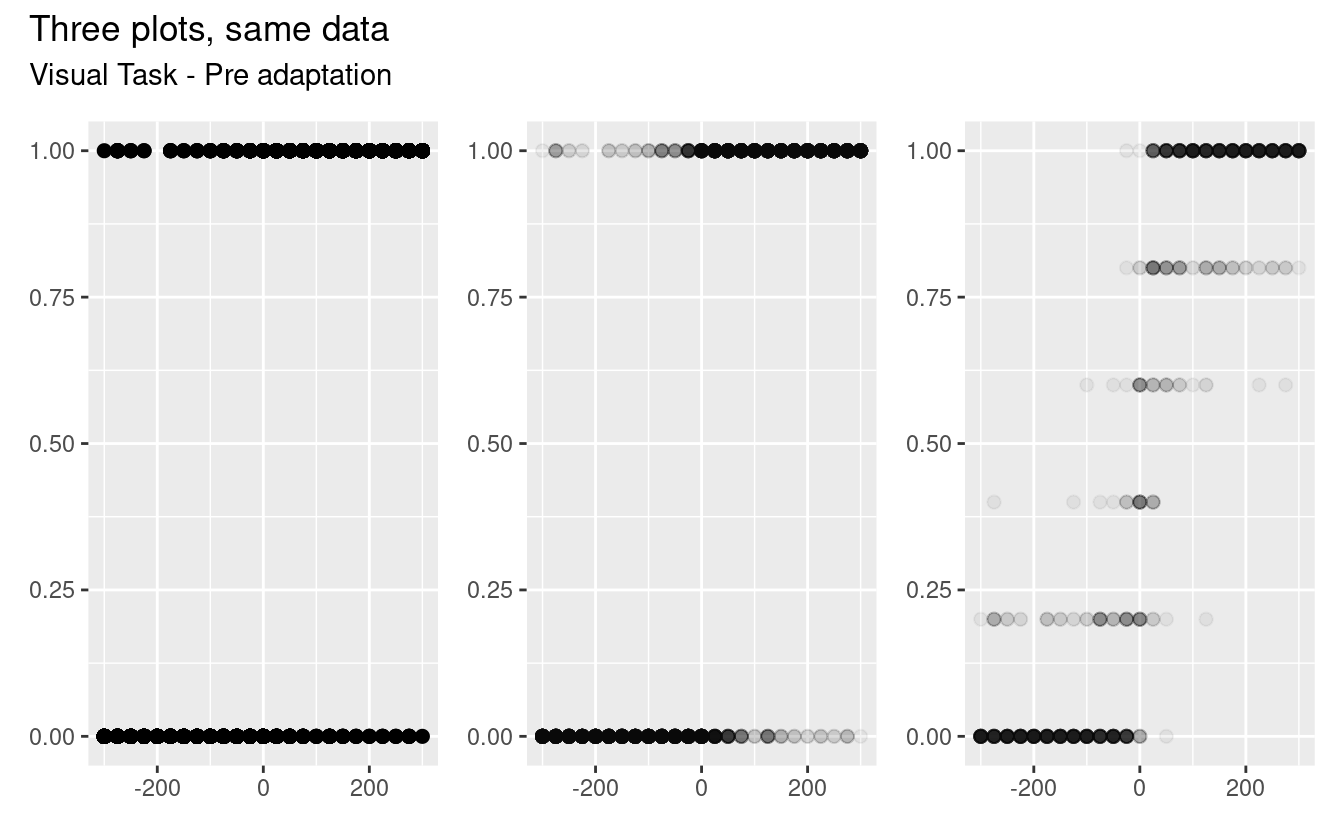
\includegraphics[width=0.7\linewidth]{020-psychometrics_files/figure-latex/ch020-simple-response-soa-plot-1} 

}

\caption{Left: Simple plot of response vs. soa value. Center: A plot of response vs. soa with transparency. Right: A plot of proportions vs. soa with transparency.}\label{fig:ch020-simple-response-soa-plot}
\end{figure}

Subjectively the right plot in figure \ref{fig:ch020-simple-response-soa-plot} is the easiest to interpret. Because of this, I will often present the observed and predicted data using the proportion of responses rather than the actual response. Proportional data also has the advantage of being bounded on the same interval as the response. For the audiovisual task, the responses can be aggregated into binomial data -- the number of positive responses for given SOA value -- which is sometimes more efficient to work with than the Bernoulli data (see table \ref{tab:ch020-av-bin-sample}). However the number of times an SOA is presented varies between the pre-adaptation and post-adaptation blocks; 5 and 3 times per SOA respectively.

\begin{table}[!h]

\caption{\label{tab:ch020-av-bin-sample}Audiovisual task with aggregated responses.}
\centering
\begin{tabular}[t]{lrrrr}
\toprule
trial & soa & n & k & proportion\\
\midrule
 & 200 & 5 & 4 & 0.80\\
\cmidrule{2-5}
 & 150 & 5 & 5 & 1.00\\
\cmidrule{2-5}
\multirow[t]{-3}{*}{\raggedright\arraybackslash pre} & -350 & 5 & 0 & 0.00\\
\cmidrule{1-5}
 & 350 & 3 & 3 & 1.00\\
\cmidrule{2-5}
 & -500 & 3 & 1 & 0.33\\
\cmidrule{2-5}
\multirow[t]{-3}{*}{\raggedright\arraybackslash post1} & -200 & 3 & 0 & 0.00\\
\bottomrule
\end{tabular}
\end{table}

Other quirks about the data pertain to the subjects. There is one younger subject that did not complete the audiovisual task, and one younger subject that did not complete the duration task. Additionally there is one older subject who's response data for the post-adaptation audiovisual task is unreasonable\footnote{By unreasonable, I mean that it is extremely unlikely that the data represents genuine responses.} (see figure \ref{fig:ch020-av-post1-O-f-CE-plot}).

\begin{figure}

{\centering 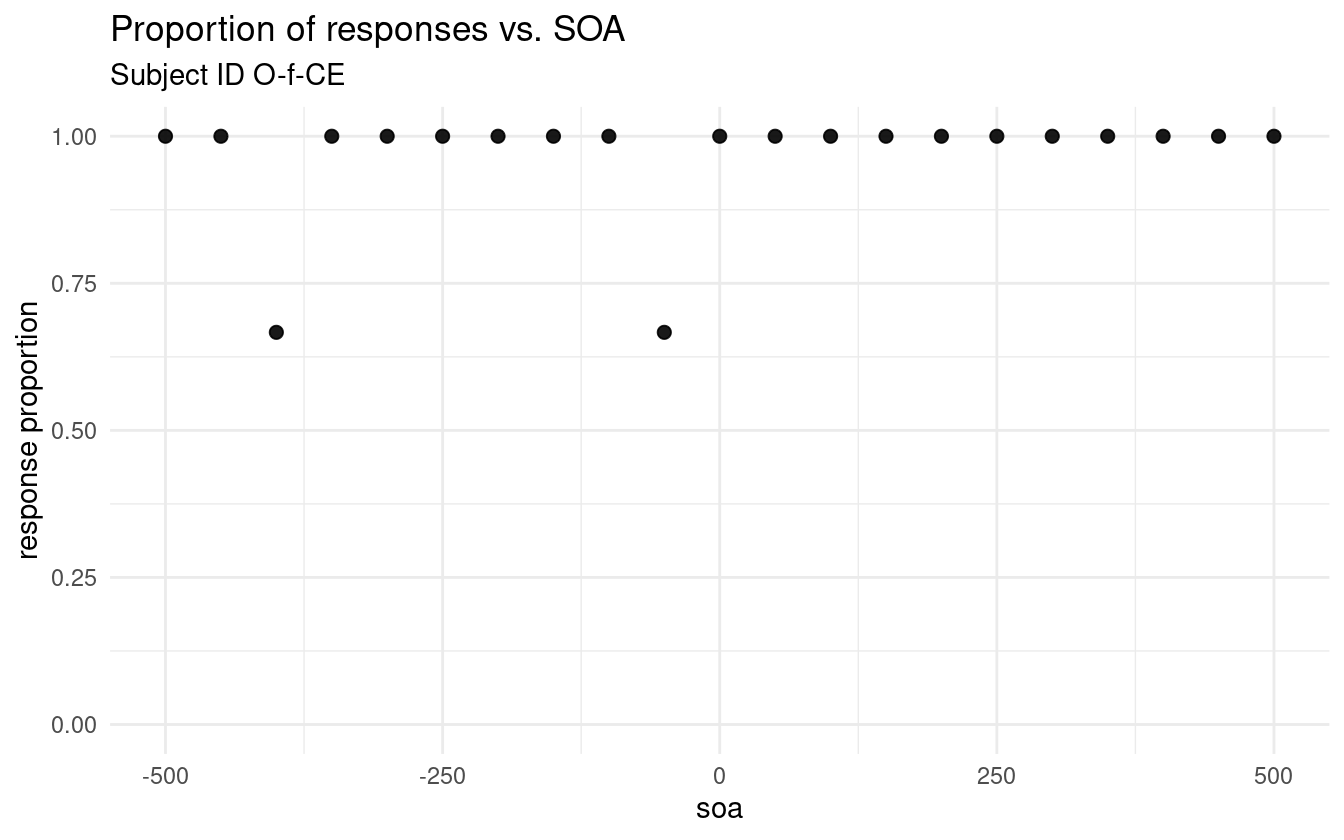
\includegraphics[width=0.7\linewidth]{020-psychometrics_files/figure-latex/ch020-av-post1-O-f-CE-plot-1} 

}

\caption{Post-adaptation response data for O-f-CE}\label{fig:ch020-av-post1-O-f-CE-plot}
\end{figure}

It is unreasonable because, of all the negative SOAs, there were only two correct responses\footnote{Correct in the sense that the perceived order matches the actual order.}. If a subject is randomly guessing the temporal order, then a naive estimate for the proportion of correct responses is 0.5. If a subject's proportion of correct responses is above 0.5, then they are doing better than random guessing. In figure \ref{fig:ch020-av-post-neg-trials} it is seen that subject O-f-CE is the only one who's proportion is below 0.5 (and by a considerable amount).

\begin{figure}

{\centering 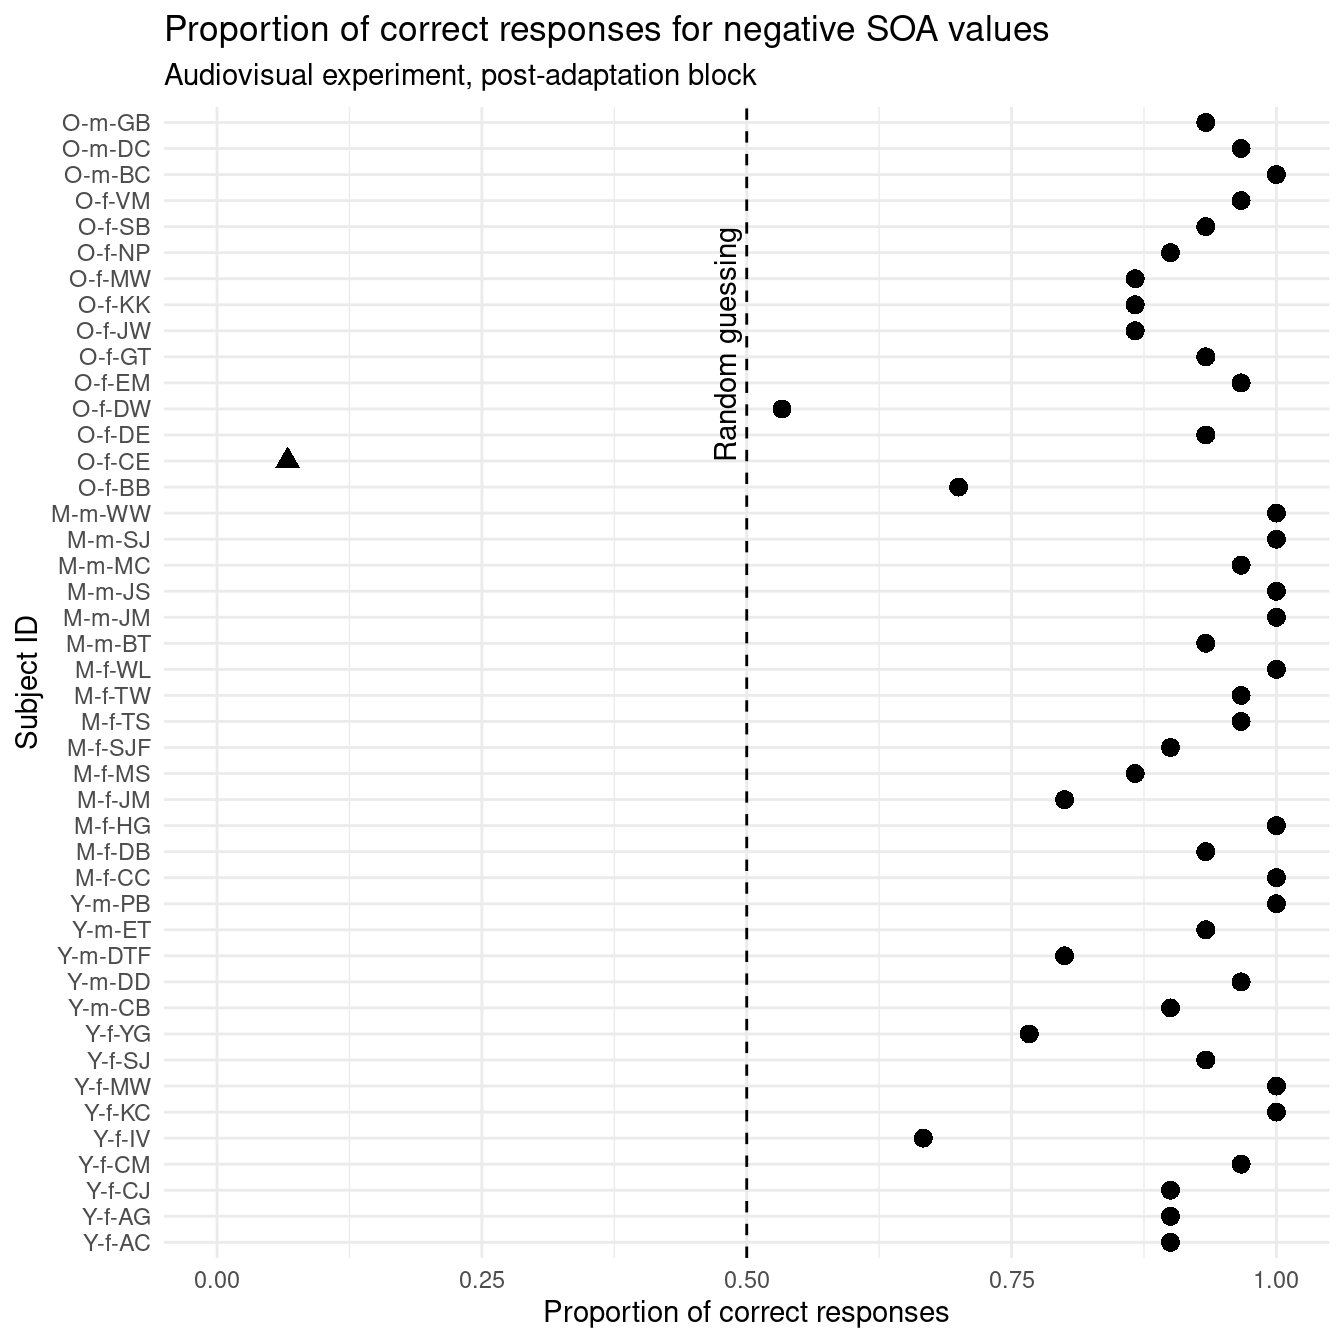
\includegraphics[width=0.7\linewidth]{020-psychometrics_files/figure-latex/ch020-av-post-neg-trials-1} 

}

\caption{Proportion of correct responses for negative SOA values during the post-adaptation audiovisual experiment.}\label{fig:ch020-av-post-neg-trials}
\end{figure}

The consequences of leaving in this experimental block in the data is considered in the \protect\hyperlink{results}{Chapter 6}, but it is a clear outlier that must be noted. When this method of detecting outliers is repeated for all tasks and blocks, then I end up with 17 records in total (see figure \ref{fig:ch020-naive-prop-outliers}), one of which is the aforementioned subject.

\begin{figure}

{\centering 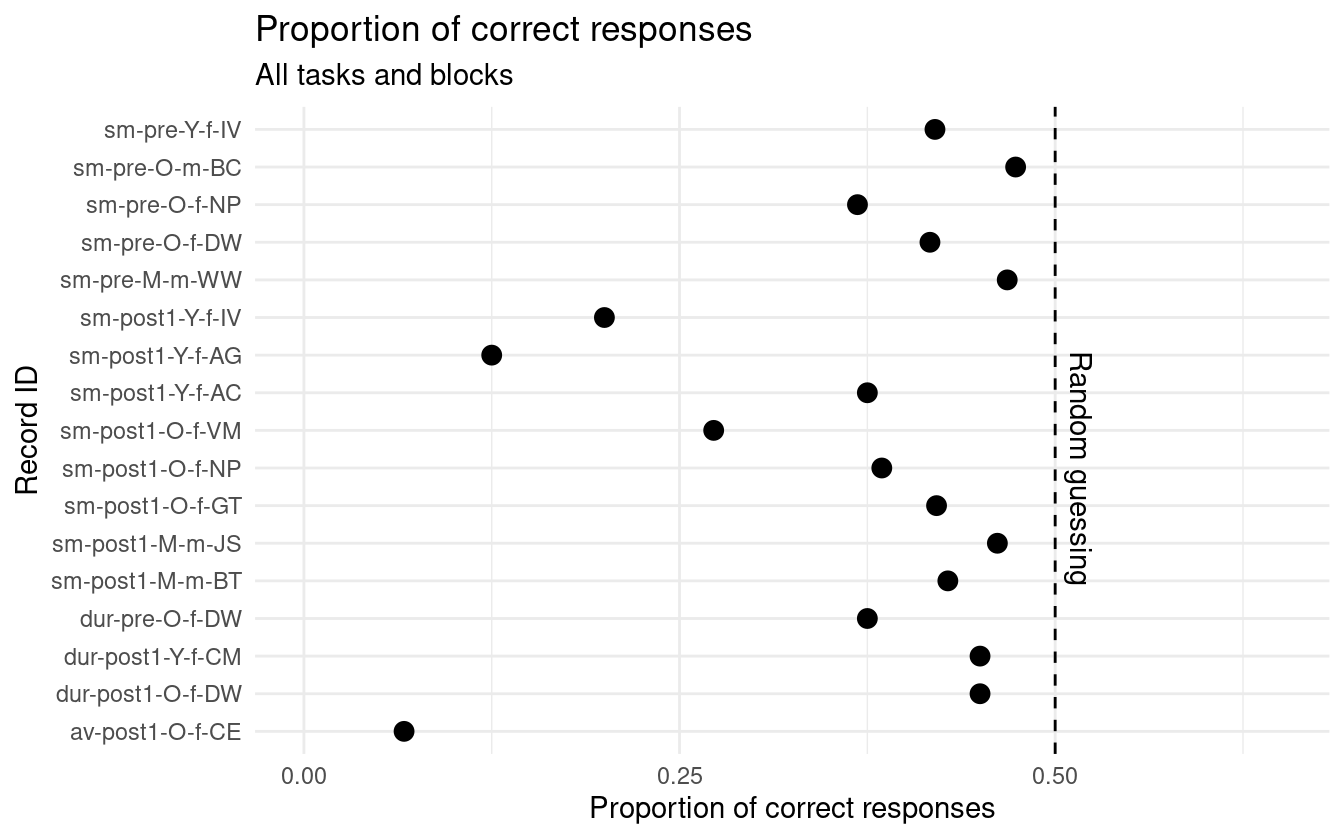
\includegraphics[width=0.7\linewidth]{020-psychometrics_files/figure-latex/ch020-naive-prop-outliers-1} 

}

\caption{Proportion of correct responses across all tasks and blocks Proportions are calculated individually for positive and negative SOAs.}\label{fig:ch020-naive-prop-outliers}
\end{figure}

Most of the records that are flagged by this method of outlier detection are from the sensorimotor task, and none are from the visual task. This may be attributed to the perceived difficulty of the task. One consequence of higher temporal sensitivity is that it is easier to determine temporal order. It may also be that determining temporal order is inherently easier for certain multisensory tasks compared to others. Since the sensorimotor task does not have fixed SOA values like the other tasks, it may be perceived as more difficult. Or perhaps the mechanisms that process tactile and visual signals are not as well coupled as those that process audio and visual signals. Once again, I'll consider the handling of the sensorimotor outliers in the results chapter.

Now that I have introduced the motivating data and some of the theory behind psychometric experiments, I am ready to introduce a Bayesian workflow for multilevel modeling of the psychometric function. If the reader is interested in a fun story, in the \protect\hyperlink{discussion}{discussion chapter} I talk about the process I went through to read in this psychometric data, clean it up, and produce a tidy data set that is ready for modeling. While data cleaning and transforming is a topic entirely to itself, it is not the main focus of this paper.

\hypertarget{workflow}{%
\chapter{Principled Bayesian Workflow}\label{workflow}}

\emph{The meat, the cheese, the entire sandwich}

Leading up to now, I haven't discussed what is a principled Bayesian workflow, nor what multilevel modeling is. I was hoping to build up the suspense. Well I hope you're now ready for the answer. A principled Bayesian workflow is a method of employing domain expertise and statistical knowledge to iteratively build a statistical model that satisfies the constraints and goals set forth by the researcher. Oh, and Bayesian techniques are used in exchange for classical ones. Maybe not worth the suspense, but the simple idea spawns a creative and descriptive way to analyze data.

What about the multilevel aspect? While I get into that more in the following sections, the concept is simple. Multilevel models should be the default. The alternatives are models with complete pooling, or models with no pooling. Pooling vs.~no pooling is a fancy way of saying that all the data is modeled as a whole, or the smallest component (group) is modeled individually. The former implies that the variation between groups is zero (all groups are the same), and the latter implies that the variation between groups is infinite (no groups are the same). Multilevel models assume that the truth is somewhere in the middle of zero and infinity. That's not a difficult thing to posit.

Hierarchical models are a specific kind of multilevel model where one or more groups are nested within a larger one. In the case of the psychometric data, there are three age groups, and within each age group are individual subjects. Multilevel modeling provides a way to quantify and apportion the variation within the data to each level in the model. For an in-depth introduction to multilevel modeling, see \citet{gelman2006data}.

There are many great resources out there for following along with an analysis of some data or problem, and much more is the abundance of tips, tricks, techniques, and testimonies to good modeling practices. The problem is that many of these prescriptions are given without context for when they are appropriate to be taken. According to \citet{betancourt2020}, this leaves ``practitioners to piece together their own model building workflows from potentially incomplete or even inconsistent heuristics.'' The concept of a principled workflow is that for any given problem, there is not, nor should there be, a default set of steps to take to get from data exploration to predictive inferences. Rather great consideration must be given to domain expertise and the questions that one is trying to answer with the data.

Since everyone asks different questions, the value of a model is not in how well it ticks the boxes of goodness-of-fit checks, but in how consistent it is with domain expertise and its ability to answer the unique set of questions. Betancourt suggests answering four questions to evaluate a model by:

\begin{enumerate}
\def\labelenumi{\arabic{enumi}.}
\tightlist
\item
  Domain Expertise Consistency - Is our model consistent with our domain expertise?
\item
  Computational Faithfulness - Will our computational tools be sufficient to accurately fit our posteriors?
\item
  Inferential Adequacy - Will our inferences provide enough information to answer our questions?
\item
  Model Adequacy - Is our model rich enough to capture the relevant structure of the true data generating process?
\end{enumerate}

Like any good Bayesian\footnote{The opposite of a Frequentist.}, much work is done before seeing the data or building a model. This may include talking with experts to gain domain knowledge or to \emph{elicit priors}. Experts may know something about a particular measure, perhaps the mean or variability of the data from years of research, and different experts may provide different estimates of a measure. The benefit of modeling in a Bayesian framework is that all prior knowledge may be incorporated into the model to be used to estimate the \emph{posterior distribution}. The same prior knowledge may also be used to check the posterior to ensure that predictions remain within physical or expert-given constraints. Consistency is key.

The computational tool I will be using to estimate the posterior is a probabilistic programming language (PPL) called Stan \citep{R-rstan} within the R programming language. Stan uses the No U-Turn Sampler (NUTS) version of Hamiltonian Monte Carlo (HMC). For a gentle introduction to Bayesian statistics and sampling methods, see \citet{bolstad2016introduction}, and for an in-depth review of HMC see \citet{betancourt2017conceptual}.

Why do we need a sampler at all? Bayesian statistics and modeling stems from Bayes theorem (Equation \eqref{eq:bayesthm}). The prior \(P(\theta)\) is some distribution over the parameter space and the likelihood \(P(X | \theta)\) is the probability of an outcome in the sample space given a value in the parameter space. To keep things simple, we generally say that the posterior is proportional to the prior times the likelihood. Why proportional? The posterior distribution is a probability distribution, which means that the sum or integral over the parameter space must evaluate to one. Because of this constraint, the denominator in \eqref{eq:bayesthm} acts as a scale factor to ensure that the posterior is valid. Often it happens that the integral in the denominator is complex or of a high dimension. In the former situation, the integral may not be possible to evaluate, and in the latter there may not be enough computational resources in the world to perform a simple grid approximation.

\begin{equation}
  P(\theta | X) = \frac{P(X | \theta)\cdot P(\theta)}{\sum_i P(X | \theta_i)} =   \frac{P(X | \theta)\cdot P(\theta)}{\int_\Omega P(X | \theta)d\theta}
  \label{eq:bayesthm}
\end{equation}

The solution is to use Markov Chain Monte Carlo (MCMC). The idea is that we can \emph{draw samples} from the posterior distribution in a way that samples proportionally to the density. This sampling is a form of approximation to the area under the curve (i.e.~an approximation to the denominator in \eqref{eq:bayesthm}). Rejection sampling \citep{gilks1992adaptive} and slice sampling \citep{neal2003slice} are basic methods for sampling from a target distribution, however they can often be inefficient\footnote{Efficiency of a sampler is related to the proportion of proposal samples that get accepted.}. NUTS is a much more complex algorithm that can be compared to a physics simulation. A massless ``particle'' is flicked in a random direction with some amount of kinetic energy in a probability field, and is stopped randomly. The stopping point is the new proposal sample. The No U-Turn part means that when the algorithm detects that the particle is turning around, it will stop so as not to return to the starting position. This sampling scheme has a much higher rate of accepted samples, and also comes with many built-in diagnostic tools that let us know when the sampler is having trouble efficiently exploring the posterior. I'll talk more about these diagnostic tools throughout the remaining sections and in \protect\hyperlink{model-checking}{chapter 4}.

The question of inferential adequacy depends on the set of questions that we are seeking to answer with the data from the psychometric experiment. The broad objective is to determine if there are any significant differences between age groups when it comes to temporal sensitivity, perceptual synchrony, and temporal recalibration, and if the task influences the results as well. The specific goals are to estimate and compare the PSS an JND across all age groups, conditions, and tasks, and determine the affect of recalibration between age groups.

For the last question, model adequacy, I will be following a set of steps proposed in \citet{betancourt2020}. The purpose of laying out these steps is not to again blindly check them off, but to force the analyst to carefully consider each point and make an \emph{informed} decision whether the step is necessary or to craft the specifics of how the step should be completed. The steps are listed in table \ref{tab:ch030-workflow-steps}. These steps are also not meant to be followed linearly. If at any point it is discovered that there is an issue in conceptual understanding or model adequacy or something else, then it is encouraged to go back to a previous step and start with a new understanding.

\begin{table}[!h]

\caption{\label{tab:ch030-workflow-steps}Principled workflow}
\centering
\begin{tabular}[t]{ll}
\toprule
Part & Step\\
\midrule
 & conceptual analysis\\
\cmidrule{2-2}
 & define observational space\\
\cmidrule{2-2}
\multirow[t]{-3}{*}{\raggedright\arraybackslash Pre-Model, Pre-Data} & construct summary statistics\\
\cmidrule{1-2}
 & develop model\\
\cmidrule{2-2}
 & construct summary functions\\
\cmidrule{2-2}
 & simulate Bayesian ensemble\\
\cmidrule{2-2}
 & prior checks\\
\cmidrule{2-2}
 & configure algorithm\\
\cmidrule{2-2}
 & fit simulated ensemble\\
\cmidrule{2-2}
 & algorithmic calibration\\
\cmidrule{2-2}
\multirow[t]{-8}{*}{\raggedright\arraybackslash Post-Model, Pre-Data} & inferential calibration\\
\cmidrule{1-2}
 & fit observed data\\
\cmidrule{2-2}
 & diagnose posterior fit\\
\cmidrule{2-2}
 & posterior retrodictive checks\\
\cmidrule{2-2}
\multirow[t]{-4}{*}{\raggedright\arraybackslash Post-Model, Post-Data} & celebrate\\
\bottomrule
\end{tabular}
\end{table}

I'll talk about each step in the first iteration, but may choose to omit steps in subsequent iterations if there are no changes. For the purposes of building a model and being concise, I will focus around the audiovisual TOJ task in this chapter, but the final model will apply similarly to the visual and duration tasks. For the sensorimotor task, the model will be modified to accept Bernoulli data as apposed to aggregated Binomial counts (described more in the next section).

\hypertarget{iter1}{%
\section{Iteration 1 (journey of a thousand miles)}\label{iter1}}

\textbf{pre-model, pre-data}

I begin the modeling process by modeling the experiment according to the description of how it occurred and how the data were collected. This first part consists of conceptual analysis, defining the observational space, and constructing summary statistics that can help us to identify issues in the model specification.

\emph{conceptual analysis}

In section \ref{toj-task} I discussed the experimental setup and data collection. To reiterate, subjects are presented with two stimuli separated by some temporal delay, and they are asked to respond as to their perception of the temporal order. There are 45 subjects with 15 each in the young, middle, and older age groups. As the SOA becomes larger in the positive direction, subjects are expected to give more ``positive'' responses, and as the SOA becomes larger in the negative direction, more ``negative'' responses are expected. By the way the experiment and responses are constructed, there is no expectation to see a reversal of this trend unless there was an issue with the subject's understanding of the directions given to them or an error in the recording device.

After the first experimental block the subjects go through a recalibration period, and repeat the experiment again. The interest is in seeing if the recalibration has an effect on temporal sensitivity and perceptual synchrony, and if the effect is different for each age group.

\emph{define observational space}

The response that subjects give during a TOJ task is recorded as a zero or a one (see section \ref{toj-task}), and their relative performance is determined by the SOA value. Let \(y\) represent the binary outcome of a trial and let \(x\) be the SOA value.

\begin{align*}
y_i &\in \lbrace 0, 1\rbrace \\
x_i &\in \mathbb{R}
\end{align*}

If the SOA values are fixed like in the audiovisual task, then the responses can be aggregated into binomial counts, \(k\).

\[
k_i, n_i \in \mathbb{Z}_0^+, k_i \le n_i
\]

In the above expression, \(\mathbb{Z}_0^+\) represents the set of non-negative integers. Notice that the number of trials \(n\) has an index variable \(i\). This is because the number of trials per SOA is not fixed between blocks. In the pre-adaptation block, there are five trials per SOA compared to three in the post-adaptation block. So if observation 32 is recorded during a ``pre'' block, \(n_{32} = 5\), and if observation 1156 is during a ``post'' block, \(n_{1156} = 3\). Of course this is assuming that each subject completed all trials in the block, but the flexibility of the indexing can manage even if they didn't.

Then there are also three categorical variables -- age group, subject ID, and trial (block). The first two are treated as factor variables\footnote{Factor variables also go by the name index variable or categorical variable}. Rather than using one-hot encoding or dummy variables, the age levels are left as categories and a coefficient is fit for each level. Among the benefits of this approach is the ease of interpretation and ease of working with the data programmatically. This is especially true at the subject level. If a dummy variables was used for all 45 subjects, we would have 44 different dummy variables to work with times the number of coefficients that make estimates at the subject level. The number of parameters in the model grows rapidly as the model complexity grows.

Age groups and individual subjects can be indexed in the same way that number of trials is indexed. \(S_i\) refers to the subject in record \(i\), and similarly \(G_i\) refers to the age group of that subject. Observation 63 is for record ID av-post1-M-f-HG, so then \(S_{63}\) is M-f-HG and \(G_{63}\) is middle\_age. Under the hood of R, these factor levels are represented as integers (e.g.~middle age group level is stored internally as the number 2).

\begin{Shaded}
\begin{Highlighting}[]
\NormalTok{(x <-}\StringTok{ }\KeywordTok{factor}\NormalTok{(}\KeywordTok{c}\NormalTok{(}\StringTok{"a"}\NormalTok{, }\StringTok{"a"}\NormalTok{, }\StringTok{"b"}\NormalTok{, }\StringTok{"c"}\NormalTok{)))}
\CommentTok{#> [1] a a b c}
\CommentTok{#> Levels: a b c}
\KeywordTok{storage.mode}\NormalTok{(x)}
\CommentTok{#> [1] "integer"}
\end{Highlighting}
\end{Shaded}

This data storage representation can later be exploited for the Stan model.

The pre- and post-adaptation categories are treated as a binary indicator referred to as \(trt\) (short for treatment) since there are only two levels in the category. In this setup, a value of 1 indicates a post-adaptation block. I chose this encoding over the reverse because the pre-adaptation block is like the baseline performance, and it seemed more appropriate to interpret the post-adaptation block as turning on some effect. Using a binary indicator in a regression setting may not be the best practice as I discuss in section \ref{iter2}.

In the Stan modeling language, data for a binomial model with subject and age group levels and treatment is specified as

\setstretch{1.0}

\begin{verbatim}
data {
  int N;        // Number of observations
  int N_S;      // Number of subject levels
  int N_G;      // Number of age group levels
  int N_T;      // Number of treatment/control groups
  int n[N];     // Trials per SOA
  int k[N];     // binomial counts
  vector[N] x;  // SOA values
  int S[N];     // Subject identifier
  int G[N];     // Age group identifier
  int trt[N];   // Treatment indicator
}
\end{verbatim}

\setstretch{2.0}

In Stan (and unlike in R), data types must be statically declared. While sometimes a nuisance, this requirement aids in something called \emph{type inference}, and also lets Stan optimize certain parts of the model.

\emph{construct summary statistics}

In order to effectively challenge the validity of the model, a set of summary statistics are constructed that help answer the questions of domain expertise consistency and model adequacy. We are studying the affects of age and temporal recalibration through the PSS and JND (see section \ref{psycho-experiments}), so it is natural to define summary statistics around these quantities to verify model consistency. Additionally the PSS and JND can be computed regardless of the model parameterization or chosen psychometric function.

By the experimental setup and recording process, it is impossible that a properly conducted block would result in a JND less than 0 (i.e.~the psychometric function is always non-decreasing), so that can be a lower limit for its threshold. On the other end it is unlikely that it will be beyond the limits of the SOA values, but even more concrete, it seems unlikely (though not impossible) that the just noticeable difference would be more than a second.

The lower bound on the JND can be further refined if we draw information from other sources. Some studies show that we cannot perceive time differences below 30 ms, and others show that an input lag as small as 100ms can impair a person's typing ability. Then according to these studies, a time delay of 100ms is enough to notice, and so a just noticeable difference should be much less than one second -- much closer to 100ms. I'll continue to use one second as an extreme estimate indicator, but will incorporate this knowledge when it comes to selecting priors.

As for the point of subjective simultaneity, it can be either positive or negative, with the belief that larger values are more rare. Some studies suggest that for audio-visual TOJ tasks, the separation between stimuli need to be as little as 20 milliseconds for subjects to be able to determine which modality came first \citep{vatakis2007influence}. Other studies suggest that our brains can detect temporal differences as small as 30 milliseconds. If these values are to be believed then we should be skeptical of PSS estimates larger than say 150 milliseconds in absolute value, just to be safe.

A histogram of computed PSS and JND values will suffice for summary statistics. We can estimate the proportion of values that fall outside of our limits defined above, and use them as indications of problems with the model fitting or conceptual understanding.

\textbf{post-model, pre-data}

It is now time to define priors for the model, while still not having looked at the {[}distribution of{]} data. The priors should be motivated by domain expertise and \emph{prior knowledge}, not the data. There are also many choices when it comes to selecting a psychometric (sigmoid) function. Common ones are logistic, Gaussian, and Weibull.

\begin{figure}

{\centering 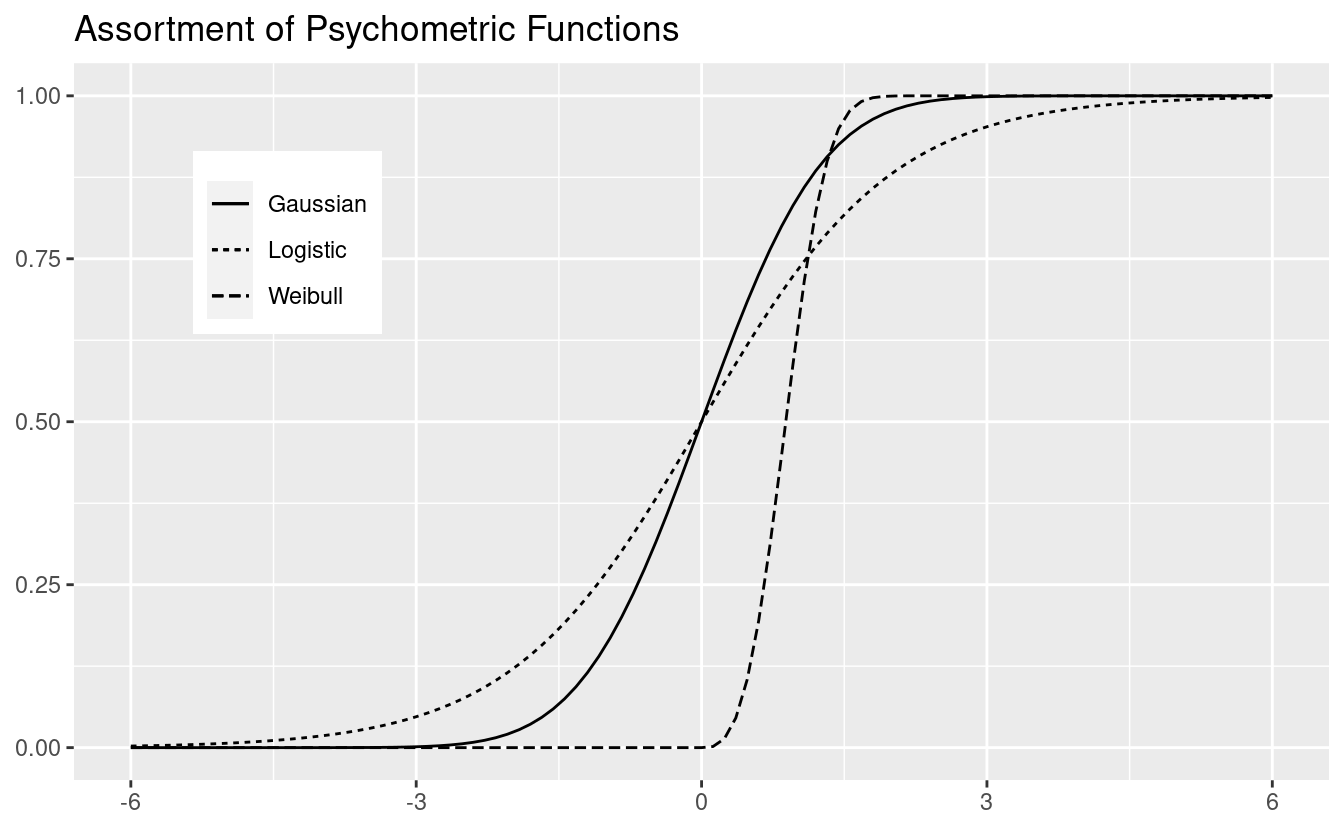
\includegraphics[width=0.7\linewidth]{030-workflow_files/figure-latex/ch031-pf-assortment-1} 

}

\caption{Assortment of psychometric functions.}\label{fig:ch031-pf-assortment}
\end{figure}

The Weibull psychometric function is more common when it comes to 2-AFC psychometric experiments where the independent variable is a stimulus intensity (non-negative) and the goal is signal detection. The data in this paper includes both positive and negative SOA values, so the Weibull is not a natural choice. In fact, because this is essentially a model for logistic regression, my first choice is the logistic function as it is the canonical choice for Binomial data. Additionally, the data in this study are reversible. The label of a positive response can be swapped with the label of a negative response and the inferences should remain the same. Since there is no natural ordering, it makes more sense for the psychometric function to be symmetric, e.g.~the logistic and Gaussian. I use symmetric loosely to mean that probability density function (PDF) is symmetric about its middle. More specifically, the distribution has zero skewness.

In practice, there is little difference in inference between the \emph{logit} and \emph{probit} links, but computationally the logit link is more efficient. I am also more familiar with working on the log-odds scale compared to the probit scale, so I make the decision to go forward with the logistic function. In \protect\hyperlink{model-checking}{chapter 4} I will show how even with a mis-specified link function, we can still achieve accurate predictions.

\emph{develop model}

Before moving on to specifying priors, I think it is appropriate to provide a little more background into generalized linear models (GLMs) and their role in working with psychometric functions. A GLM allows the linear model to be related to the outcome variable via a \emph{link} function. An example of this is the logit link - the inverse of the logistic function. The logistic function, \(F\), takes \(x \in \mathbb{R}\) and constrains the output to be in \((0, 1)\).

\begin{equation}
  F(\theta) = \frac{1}{1 + \exp\left(-\theta\right)}
  \label{eq:logistic}
\end{equation}

Since \(F\) is a strictly increasing and continuous function, it has an inverse, and the link for \eqref{eq:logistic} is the log-odds or logit function.

\begin{equation}
  F^{-1}(\pi) = \mathrm{logit}(\pi) = \ln\left(\frac{\pi}{1 - \pi}\right)
  \label{eq:logit}
\end{equation}

By taking \((F^{-1} \circ F)(\theta)\) we can arrive at a relationship that is linear in \(\theta\).

\begin{align*}
  \pi = F(\theta) \Longleftrightarrow F^{-1}(\pi) &= F^{-1}(F(\theta)) \\
  & = \ln\left(\frac{F(\theta)}{1 - F(\theta)}\right) \\
  &= \ln(F(\theta)) - \ln(1 - F(\theta)) \\
  &= \ln\left(\frac{1}{1 + \exp(-\theta)}\right) - \ln\left(\frac{\exp(-\theta)}{1 + \exp(-\theta)}\right) \\
  &= - \ln(1 + \exp(-\theta)) - \ln(\exp(-\theta)) + \ln(1 + \exp(-\theta)) \\
  &= - \ln(\exp(-\theta)) \\
  &= \theta
\end{align*}

The purpose of all this setup is to show that a model for the psychometric function can be specified using a linear predictor, \(\theta\). Given a simple slope-intercept model, one would typically write the linear predictor as

\begin{equation}
  \theta = \alpha + \beta x
  \label{eq:linearform1}
\end{equation}

This isn't the only acceptable form; it could be written in the centered parameterization

\begin{equation}
  \theta = \beta(x - a)
  \label{eq:linearform2}
\end{equation}

Both parameterizations will describe the same geometry, so why should it matter which form is chosen? Clearly the interpretation of the parameters change between the two models, but the reason becomes clear when you consider how the linear model relates back to the physical properties that the psychometric model describes. Take equation \eqref{eq:linearform1}, substitute it in to \eqref{eq:logistic}, and then take the logit of both sides

\begin{equation}
  \mathrm{logit}(\pi) = \alpha+\beta x
  \label{eq:pfform1}
\end{equation}

Now recall that the PSS is defined as the SOA values such that the response probability, \(\pi\), is \(0.5\). Substituting \(\pi = 0.5\) into \eqref{eq:pfform1} and solving for \(x\) yields

\[
pss = -\frac{\alpha}{\beta}
\]

Similarly, the JND is defined as the difference between the SOA value at the 84\% level and the PSS. Substituting \(\pi = 0.84\) into \eqref{eq:pfform1}, solving for \(x\), and subtracting off the pss yields

\begin{equation}
  jnd = \frac{\mathrm{logit}(0.84)}{\beta}
  \label{eq:jnd1}
\end{equation}

From the conceptual analysis, it is easy to define priors for the PSS and JND, but then how does one set the priors for \(\alpha\) and \(\beta\)? Let's say the prior for the just noticeable difference is \(jnd \sim \pi_j\). Then the prior for \(\beta\) would be

\[
\beta \sim \frac{\mathrm{logit}(0.84)}{\pi_j}
\]

The log-normal distribution has a nice property where its multiplicative inverse is still a log-normal distribution. We could let \(\pi_j = \mathrm{Lognormal}(\mu, \sigma^2)\) and then \(\beta\) would be distributed as

\[
\beta \sim \mathrm{Lognormal}(-\mu + \ln(\mathrm{logit}(0.84)), \sigma^2)
\]

This is acceptable, as it was determined last chapter that the slope must always be positive, and a log-normal distribution constrains the support to postive real numbers. Next suppose that the prior distribution for the PSS is \(pss \sim \pi_p\). Then the prior for \(\alpha\) is

\[
\alpha \sim -\pi_p \cdot \beta
\]

If \(\pi_p\) is set to a log-normal distribution as well, then \(\pi_p \cdot \beta\) would also be log-normal, but there is still the problem of the negative sign. If \(\alpha\) is always negative, then the PSS will also always be negative, which is certainly not always true. Furthermore, I don't want to \emph{a priori} put more weight on positive PSS values compared to negative ones, for which a lognormal distribution would not do.

Let's now go back and consider using equation \eqref{eq:linearform2} and repeat the above process.

\begin{equation}
  \mathrm{logit}(\pi) = \beta(x - a)
  \label{eq:pfform2}
\end{equation}

The just noticeable difference is still given by \eqref{eq:jnd1} and so the same method for choosing a prior can be used, but the PSS is now given by

\[
pss = \alpha
\]

This is a fortunate consequence of using \eqref{eq:linearform2} because now the JND only depends on \(\beta\) and the PSS only depends on \(\alpha\), and now \(\alpha\) can literally be interpreted as the PSS of the estimated psychometric function! Also thrown in is the ability to set a prior for \(\alpha\) that is symmetric around \(0\) like a Gaussian distribution.

This also brings me to point out the first benefit of using a modeling language like Stan over others. For fitting GLMs in R, there are a handful of functions that utilize MLE like \texttt{stats::glm} and others that use Bayesian methods like \texttt{rstanarm::stan\_glm} and \texttt{arm::bayesglm} \citep{R-rstanarm, R-arm}. Each of these functions requires the linear predictor to be in the form of \eqref{eq:linearform1}. The \texttt{stan\_glm} function actually uses Stan in the backend to fit a model, but is limited to priors from the Student t family of distributions. By writing the model directly in Stan, the linear model can be parameterized in any way and with any prior distribution, and so allows for much more expressive modeling - a key aspect of this principled workflow.

For the first iteration of this model, I am going to start with the simplest model that captures the structure of the data without including information about age group, treatment, or subject. Here is a simple model that draws information from the conceptual analysis.

\begin{align*}
  k_i &\sim \mathrm{Binomial}(n_i, p_i) \\
  \mathrm{logit}(p_i) &= \beta ( x_i - \alpha )
\end{align*}

Since I am using the linear model from \eqref{eq:linearform2}, setting the priors for \(\alpha\) and \(\beta\) is relatively straightforward. The PSS can be positive or negative without any expected bias towards either, so a symmetric distribution like the Gaussian is a fine choice for \(\alpha\) without having any other knowledge about the distribution of PSS values. Since I said earlier that a PSS value more than 150ms in absolute value is unlikely, I can define a Gaussian prior such that \(P(|pss| > 0.150) \approx 0.01\). Since the prior does not need to be exact, the following mean and variance suffice

\[
pss \sim \mathcal{N}(0, 0.06^2) \Longleftrightarrow \alpha \sim \mathcal{N}(0, 0.06^2)
\]

For the just noticeable difference, I will continue to use the log-normal distribution because it is constrained to positive values and has the nice reciprocal property. The JND is expected to be close to 100ms and extremely unlikely to exceed 1 second. This implies a prior such that the mean is around 100ms and the bulk of the distribution is below 1 second - i.e.~\(E[X] \approx 0.100\) and \(P(X < 1) \approx 0.99\). This requires solving a system of nonlinear equations in two variables

\[
\begin{cases}
E[X] = 0.100 = \exp\left(\mu + \sigma^2 / 2\right) \\
P(X < 1) = 0.99 = 0.5 + 0.5 \cdot \mathrm{erf}\left[\frac{\ln (1) - \mu}{\sqrt{2} \cdot \sigma}\right]
\end{cases}
\]

This nonlinear system can be solved using Stan's algebraic solver.

\begin{verbatim}
functions {
  vector system(vector y, vector theta, real[] x_r, int[] x_i) {
    vector[2] z;
    z[1] = exp(y[1] + y[2]^2 / 2) - theta[1];
    z[2] = 0.5 + 0.5 * erf(-y[1] / (sqrt(2) * y[2])) - theta[2];
    return z;
  }
}
transformed data {
  vector[2] y_guess = [1, 1]';
  real x_r[0];
  int x_i[0];
}
transformed parameters {
  vector[2] theta = [0.100, 0.99]';
  vector[2] y;
  y = algebra_solver(system, y_guess, theta, x_r, x_i);
}
\end{verbatim}

\begin{Shaded}
\begin{Highlighting}[]
\NormalTok{fit <-}\StringTok{ }\KeywordTok{sampling}\NormalTok{(prior_jnd, }\DataTypeTok{iter=}\DecValTok{1}\NormalTok{, }\DataTypeTok{warmup=}\DecValTok{0}\NormalTok{, }\DataTypeTok{chains=}\DecValTok{1}\NormalTok{, }\DataTypeTok{refresh=}\DecValTok{0}\NormalTok{,}
                \DataTypeTok{seed=}\DecValTok{31}\NormalTok{, }\DataTypeTok{algorithm=}\StringTok{"Fixed_param"}\NormalTok{)}
\NormalTok{sol <-}\StringTok{ }\KeywordTok{extract}\NormalTok{(fit)}
\NormalTok{sol}\OperatorTok{$}\NormalTok{y}
\CommentTok{#>           }
\CommentTok{#> iterations   [,1]  [,2]}
\CommentTok{#>       [1,] -7.501 3.225}
\end{Highlighting}
\end{Shaded}

The solver has determined that \(\mathrm{Lognormal}(-7.5, 3.2^2)\) is the appropriate prior. However, simulating some values from this distribution produces a lot of extremely small values (\(<10^{-5}\)) and a few extremely large values (\(\approx 10^2\)). This is because the expected value of a log-normal random variable depends on both the mean and standard deviation. If the median is used in place for the mean, then a more acceptable prior may be determined.

\begin{Shaded}
\begin{Highlighting}[]
\NormalTok{fit <-}\StringTok{ }\KeywordTok{sampling}\NormalTok{(prior_jnd_using_median, }\DataTypeTok{iter=}\DecValTok{1}\NormalTok{, }\DataTypeTok{warmup=}\DecValTok{0}\NormalTok{, }\DataTypeTok{chains=}\DecValTok{1}\NormalTok{, }\DataTypeTok{refresh=}\DecValTok{0}\NormalTok{,}
                \DataTypeTok{seed=}\DecValTok{31}\NormalTok{, }\DataTypeTok{algorithm=}\StringTok{"Fixed_param"}\NormalTok{)}
\NormalTok{sol <-}\StringTok{ }\KeywordTok{extract}\NormalTok{(fit)}
\NormalTok{sol}\OperatorTok{$}\NormalTok{y}
\CommentTok{#>           }
\CommentTok{#> iterations   [,1]   [,2]}
\CommentTok{#>       [1,] -2.303 0.9898}
\end{Highlighting}
\end{Shaded}

Sampling from a log-normal distribution with these parameters and plotting the histogram shows no inconsistency with the domain expertise.

\begin{center}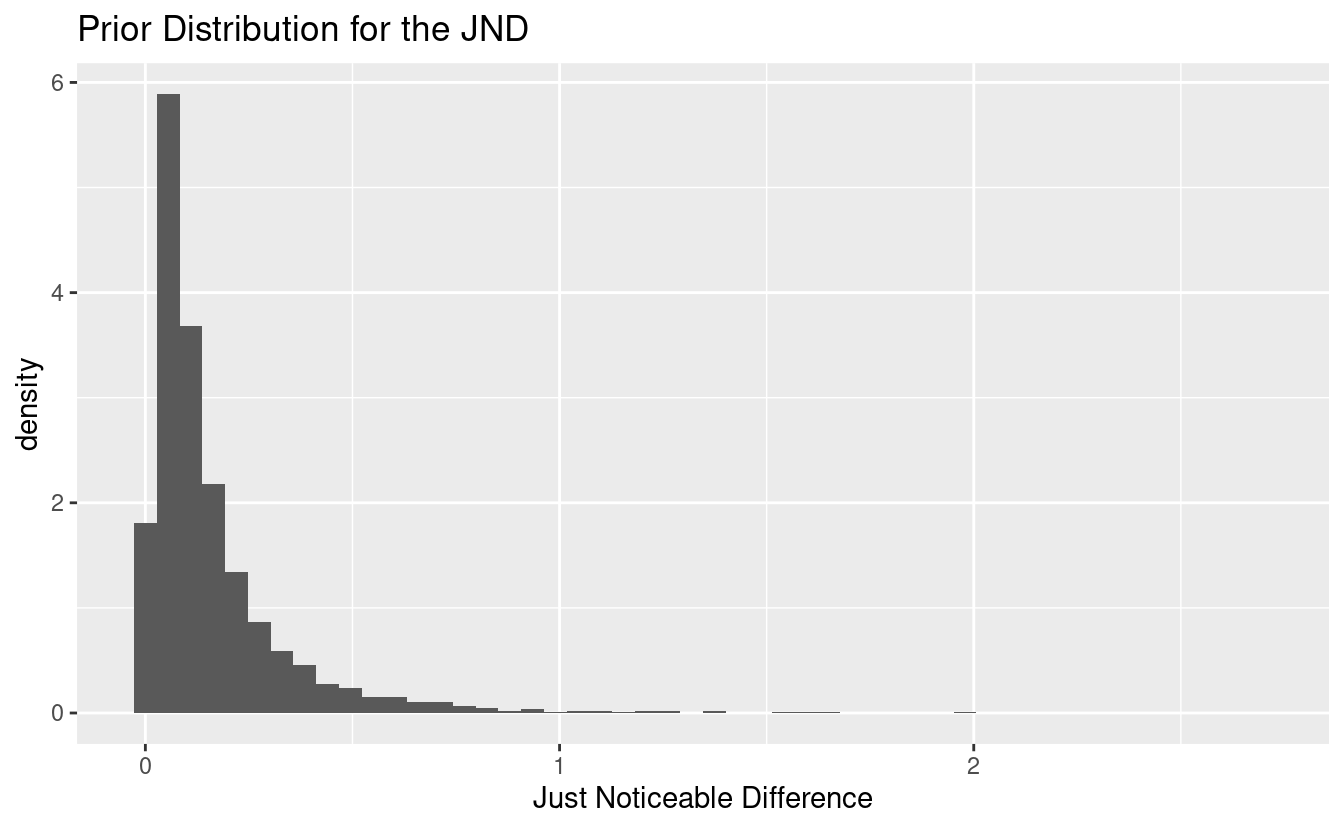
\includegraphics[width=0.7\linewidth]{030-workflow_files/figure-latex/ch031-Risky-Lion-1} \end{center}

So now with a prior for the JND, the prior for \(\beta\) can be determined.

\[
jnd \sim \mathrm{Lognormal}(-2.3, 0.99^2) \Longleftrightarrow \frac{1}{jnd} \sim \mathrm{Lognormal}(2.3, 0.99^2)
\]

and

\[
\beta = \frac{\mathrm{logit}(0.84)}{jnd} \sim \mathrm{Lognormal}(2.8, 0.99^2)
\]

The priors do not need to be too exact. Rounding the parameters for \(\beta\), the simple model is written below.

\begin{align*}
  k_i &\sim \mathrm{Binomial}(n_i, p_i) \\
  \mathrm{logit}(p_i) &= \beta ( x_i - \alpha ) \\
  \alpha &\sim \mathcal{N}(0, 0.06^2) \\
  \beta &\sim \mathrm{Lognormal}(3, 1^2)
\end{align*}

As a final check before moving on to the next step, I can simulate values from \(\alpha\) and \(\beta\) and plot the distribution of psychometric functions. This check is valuable as the interaction between the two isn't always predictable.

\begin{figure}

{\centering 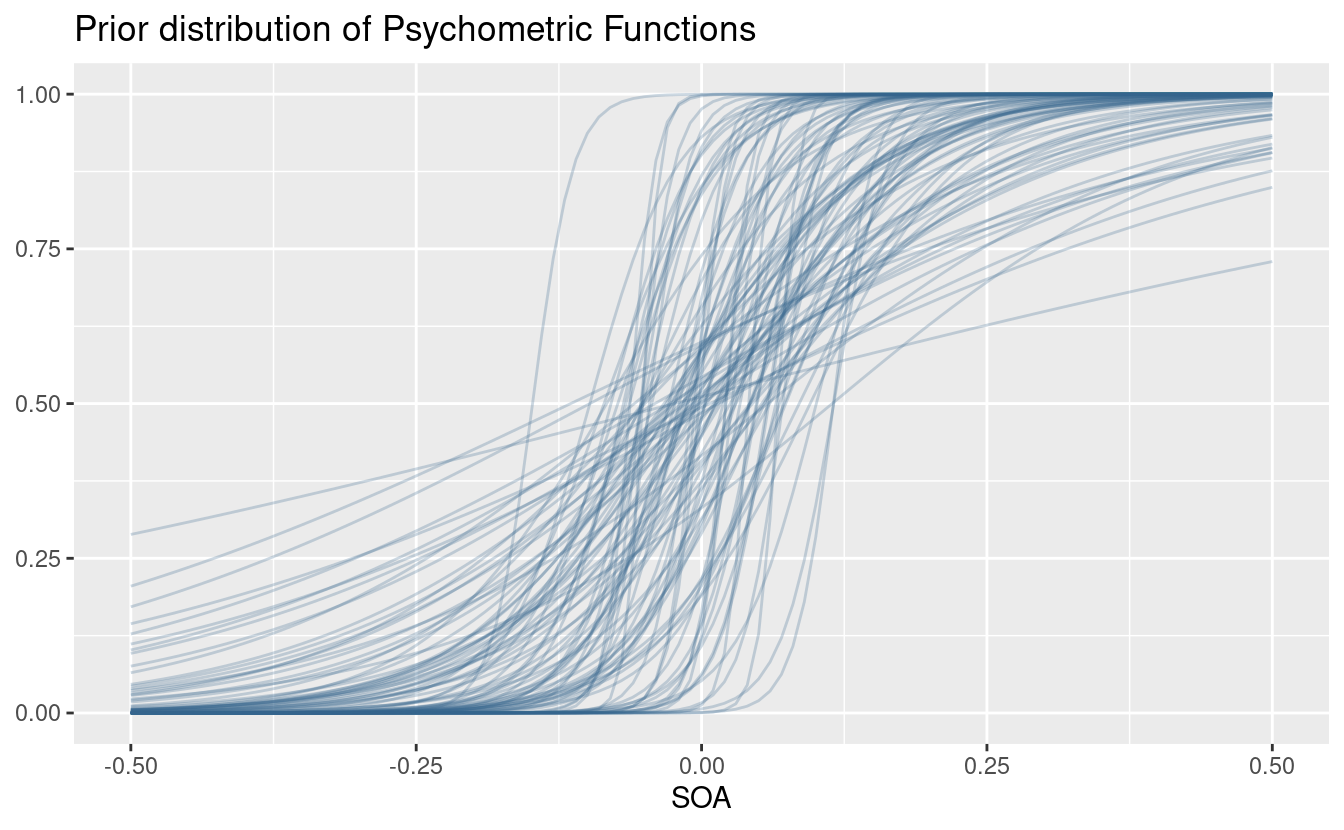
\includegraphics[width=0.7\linewidth]{030-workflow_files/figure-latex/ch030-prior-pf-plot-1} 

}

\caption{Prior distribution of psychometric functions using the priors for alpha and beta.}\label{fig:ch030-prior-pf-plot}
\end{figure}

Figure \ref{fig:ch030-prior-pf-plot} shows the distribution of prior psychometric functions. There are a few very steep and very shallow curves, but the majority fall within a range that appears likely. Additionally most of the PSS values are within \(\pm 0.1\) with room to allow for some larger values.

\emph{construct summary functions}

Whew! that was a lot of work to define the priors for just two parameters. Thankfully going forward not as much work will need to be done to expand the model. The next step is to construct any relevant summary functions. Since the distribution of posterior PSS and JND values are needed for the summary statistics, it will be nice to have a function that can take in the posterior samples for \(\alpha\) and \(\beta\) and return the PSS and JND values. I'll define \(Q\) as a more general function that takes in the two parameters and a probability, \(\pi\), and returns the distribution of SOA values at \(\pi\).

\begin{equation}
  Q(\pi; \alpha, \beta) = \frac{\mathrm{logit(\pi)}}{\beta} + \alpha
  \label{eq:summfun1}
\end{equation}

With \(Q\), the PSS and JND can be calculated as

\begin{align}
  pss &= Q(0.5) \\
  jnd &= Q(0.84) - Q(0.5)
\end{align}

\emph{simulate Bayesian ensemble}

\emph{prior checks}

\emph{configure algorithm}

\emph{fit simulated ensemble}

\emph{algorithmic calibration}

\emph{inferential calibration}

\textbf{post-model, post-data}

\emph{fit observed data}

\emph{diagnose posterior fit}

\emph{posterior retrodictive checks}

\hypertarget{iter2}{%
\section{Iteration 2 (electric boogaloo)}\label{iter2}}

\textbf{pre-model, pre-data}

\emph{conceptual analysis}

\emph{define observational space}

\emph{construct summary statistics}

\textbf{post-model, pre-data}

\emph{develop model}

\emph{construct summary functions}

\emph{simulate Bayesian ensemble}

\emph{prior checks}

\emph{configure algorithm}

\emph{fit simulated ensemble}

\emph{algorithmic calibration}

\emph{inferential calibration}

\textbf{post-model, post-data}

\emph{fit observed data}

\emph{diagnose posterior fit}

\emph{posterior retrodictive checks}

\hypertarget{iter3}{%
\section{Iteration 3 (the one for me)}\label{iter3}}

\textbf{pre-model, pre-data}

\emph{conceptual analysis}

\emph{define observational space}

\emph{construct summary statistics}

\textbf{post-model, pre-data}

\emph{develop model}

\emph{construct summary functions}

\emph{simulate Bayesian ensemble}

\emph{prior checks}

\emph{configure algorithm}

\emph{fit simulated ensemble}

\emph{algorithmic calibration}

\emph{inferential calibration}

\textbf{post-model, post-data}

\emph{fit observed data}

\emph{diagnose posterior fit}

\emph{posterior retrodictive checks}

\hypertarget{iter4}{%
\section{Iteration 4 (what's one more)}\label{iter4}}

\textbf{pre-model, pre-data}

\emph{conceptual analysis}

\emph{define observational space}

\emph{construct summary statistics}

\textbf{post-model, pre-data}

\emph{develop model}

\emph{construct summary functions}

\emph{simulate Bayesian ensemble}

\emph{prior checks}

\emph{configure algorithm}

\emph{fit simulated ensemble}

\emph{algorithmic calibration}

\emph{inferential calibration}

\textbf{post-model, post-data}

\emph{fit observed data}

\emph{diagnose posterior fit}

\emph{posterior retrodictive checks}

\hypertarget{iter5}{%
\section{Iteration 5 (final\_final\_draft\_2.pdf)}\label{iter5}}

\textbf{pre-model, pre-data}

\emph{conceptual analysis}

\emph{define observational space}

\emph{construct summary statistics}

\textbf{post-model, pre-data}

\emph{develop model}

\emph{construct summary functions}

\emph{simulate Bayesian ensemble}

\emph{prior checks}

\emph{configure algorithm}

\emph{fit simulated ensemble}

\emph{algorithmic calibration}

\emph{inferential calibration}

\textbf{post-model, post-data}

\emph{fit observed data}

\emph{diagnose posterior fit}

\emph{posterior retrodictive checks}

\hypertarget{celebrate}{%
\section{Celebrate}\label{celebrate}}

\emph{celebrate}

\hypertarget{model-checking}{%
\chapter{Model Checking}\label{model-checking}}

\begin{itemize}
\tightlist
\item
  Diagnostics
\item
  Simulation study (bigsimr?)
\item
  Consequence of using ``wrong'' model

  \begin{itemize}
  \tightlist
  \item
    Simulate logistic data and fit with probit link
  \end{itemize}
\end{itemize}

\hypertarget{predictive-inferences}{%
\chapter{Predictive Inference}\label{predictive-inferences}}

\hypertarget{results}{%
\chapter{Psychometric Results}\label{results}}

\hypertarget{discussion}{%
\chapter{Discussion}\label{discussion}}

\hypertarget{conclusion}{%
\chapter{Conclusion}\label{conclusion}}

The real story of developing this psychometric model (the one here and not in the workflow section) is more revealing of the real struggles of performing data analysis than the principled workflow would let on. Often I found myself putting in vast amounts of unnecessary work - but necessary for me to do in order to realize that it is unnecessary - just because I hadn't yet learned what the likely paths to take were. On a more personal level, my struggles were not ever really in developing a model or coding it up - in fact I could tinker with a program for hours, improving it in this way or that. For me, programming was a puzzle and an art, and I internalized the idea that I could figure out any numerical task given enough time and focus. To the contrary, I believed that writing was a chore, that writing this thesis would be like trying to dam up all the deltas in an attempt to keep the main river on course.

I think of learning mathematics as learning a puzzle game. The first few puzzles are easy, but then get progressively harder. But even as the puzzles get harder, your intuitive understanding of the game improves, and you can throw away the obviously poor moves from consideration, and try paths that are more likely to move you in the direction of the correct solution. I started my journey towards obtaining a Master of Science in Statistics precisely because I knew that I could obtain a more intuitive understanding of the quantitative world that I live in, and pick up some new tools along the way to create and solve more impressive puzzles.

\hypertarget{appendix-appendix}{%
\appendix}


\hypertarget{supplementary-code}{%
\chapter{Supplementary Code}\label{supplementary-code}}

One model, Three Implementations. There are a few ways to specify a hierarchical model in R. Below I describe three common frameworks that require varying levels of mathematical and programmatic competence. Frameworks with lower barriers for entry are great for researchers in many fields, but they lack fine control over the parameters in a model. As the framework complexity increases, so too does the ability to generate complex models that are typically not possible.

Novice
\setstretch{1.0}

\begin{Shaded}
\begin{Highlighting}[]
\KeywordTok{library}\NormalTok{(rstanarm)}
\KeywordTok{stan_glmer}\NormalTok{(}\KeywordTok{cbind}\NormalTok{(k, n}\OperatorTok{-}\NormalTok{k) }\OperatorTok{~}\StringTok{ }\DecValTok{1} \OperatorTok{+}\StringTok{ }\NormalTok{x }\OperatorTok{+}\StringTok{ }\NormalTok{(}\DecValTok{1} \OperatorTok{+}\StringTok{ }\NormalTok{x }\OperatorTok{|}\StringTok{ }\NormalTok{G1) }\OperatorTok{+}\StringTok{ }\NormalTok{(}\DecValTok{1} \OperatorTok{+}\StringTok{ }\NormalTok{x }\OperatorTok{|}\StringTok{ }\NormalTok{G2), }
           \DataTypeTok{family =} \KeywordTok{binomial}\NormalTok{(}\DataTypeTok{link =} \StringTok{"logit"}\NormalTok{),}
           \DataTypeTok{data =}\NormalTok{ dat)}
\end{Highlighting}
\end{Shaded}

\setstretch{2.0}

Intermediate

\setstretch{1.0}

\begin{Shaded}
\begin{Highlighting}[]
\KeywordTok{library}\NormalTok{(rethinking)}
\KeywordTok{ulam}\NormalTok{(}\KeywordTok{alist}\NormalTok{(}
\NormalTok{  k }\OperatorTok{~}\StringTok{ }\KeywordTok{binomial}\NormalTok{(n, pi)}
  \KeywordTok{logit}\NormalTok{(pi) <-}\StringTok{ }\NormalTok{(a }\OperatorTok{+}\StringTok{ }\NormalTok{aG1[G1] }\OperatorTok{+}\StringTok{ }\NormalTok{aG2[G2]) }\OperatorTok{+}\StringTok{ }\NormalTok{(b }\OperatorTok{+}\StringTok{ }\NormalTok{bG1[G1] }\OperatorTok{+}\StringTok{ }\NormalTok{bG2[G2]) }\OperatorTok{*}\StringTok{ }\NormalTok{x,}
  
\NormalTok{  a }\OperatorTok{~}\StringTok{ }\KeywordTok{normal}\NormalTok{(}\DecValTok{0}\NormalTok{, }\DecValTok{10}\NormalTok{),}
\NormalTok{  aG1[G1] }\OperatorTok{~}\StringTok{ }\KeywordTok{normal}\NormalTok{(}\DecValTok{0}\NormalTok{, sd_aG1),}
\NormalTok{  aG2[G2] }\OperatorTok{~}\StringTok{ }\KeywordTok{normal}\NormalTok{(}\DecValTok{0}\NormalTok{, sd_aG2),}
  \KeywordTok{c}\NormalTok{(sd_aG1, sd_aG2) }\OperatorTok{~}\StringTok{ }\KeywordTok{half_cauchy}\NormalTok{(}\DecValTok{0}\NormalTok{, }\DecValTok{10}\NormalTok{),}

\NormalTok{  b }\OperatorTok{~}\StringTok{ }\KeywordTok{normal}\NormalTok{(}\DecValTok{0}\NormalTok{, }\DecValTok{10}\NormalTok{),}
\NormalTok{  bG1[G1] }\OperatorTok{~}\StringTok{ }\KeywordTok{normal}\NormalTok{(}\DecValTok{0}\NormalTok{, sd_bG1),}
\NormalTok{  bG2[G2] }\OperatorTok{~}\StringTok{ }\KeywordTok{normal}\NormalTok{(}\DecValTok{0}\NormalTok{, sd_bG2),}
  \KeywordTok{c}\NormalTok{(sd_bG1, sd_bG2) }\OperatorTok{~}\StringTok{ }\KeywordTok{half_cauchy}\NormalTok{(}\DecValTok{0}\NormalTok{, }\DecValTok{10}\NormalTok{)}
\NormalTok{), }\DataTypeTok{data =}\NormalTok{ dat, }\DataTypeTok{log_lik =} \OtherTok{TRUE}\NormalTok{)}
\end{Highlighting}
\end{Shaded}

\setstretch{2.0}

Advanced

\setstretch{1.0}

\begin{verbatim}
data{
    int<lower=0> N;
    int<lower=0> N_G1;
    int<lower=0> N_G2;
    int n[N];
    int k[N];
    int G1[N];
    int G2[N];
    vector[N] x;
}
parameters{
    real a;
    vector[N_G1] aG1;
    vector[N_G2] aG2;
    real b;
    vector[N_G1] bG1;
    vector[N_G2] bG2;
    real<lower=0> sd_aG1;
    real<lower=0> sd_aG2;
    real<lower=0> sd_bG1;
    real<lower=0> sd_bG2;
}
model{
    vector[N] p;
    a   ~ normal(0, 10);
    aG1 ~ normal(0, sd_aG1);
    aG2 ~ normal(0, sd_aG2);
    b   ~ normal(0, 10);
    bG1 ~ normal(0, sd_bG1);
    bG2 ~ normal(0, sd_bG2);
    sd_aG1 ~ cauchy(0, 10);
    sd_aG2 ~ cauchy(0, 10);
    sd_bG1 ~ cauchy(0, 10);
    sd_bG2 ~ cauchy(0, 10);
    for (i in 1:N) {
        p[i] = (a + aG1[G1[i]] + aG2[G2[i]]) + (b + bG1[G1[i]] + bG2[G2[i]]) * x[i];
    }
    k ~ binomial_logit(n , p);
}
\end{verbatim}

\setstretch{2.0}

\setstretch{1.0}
%==============================================================================26
\backmatter
%==============================================================================27
\bibliography{bibliography.bib}
%==============================================================================28
% Place here anything that you would like to come
% after the appendix, references, etc
%==============================================================================29
\end{document}
